\begin{figure}[ht!]
	\centering
	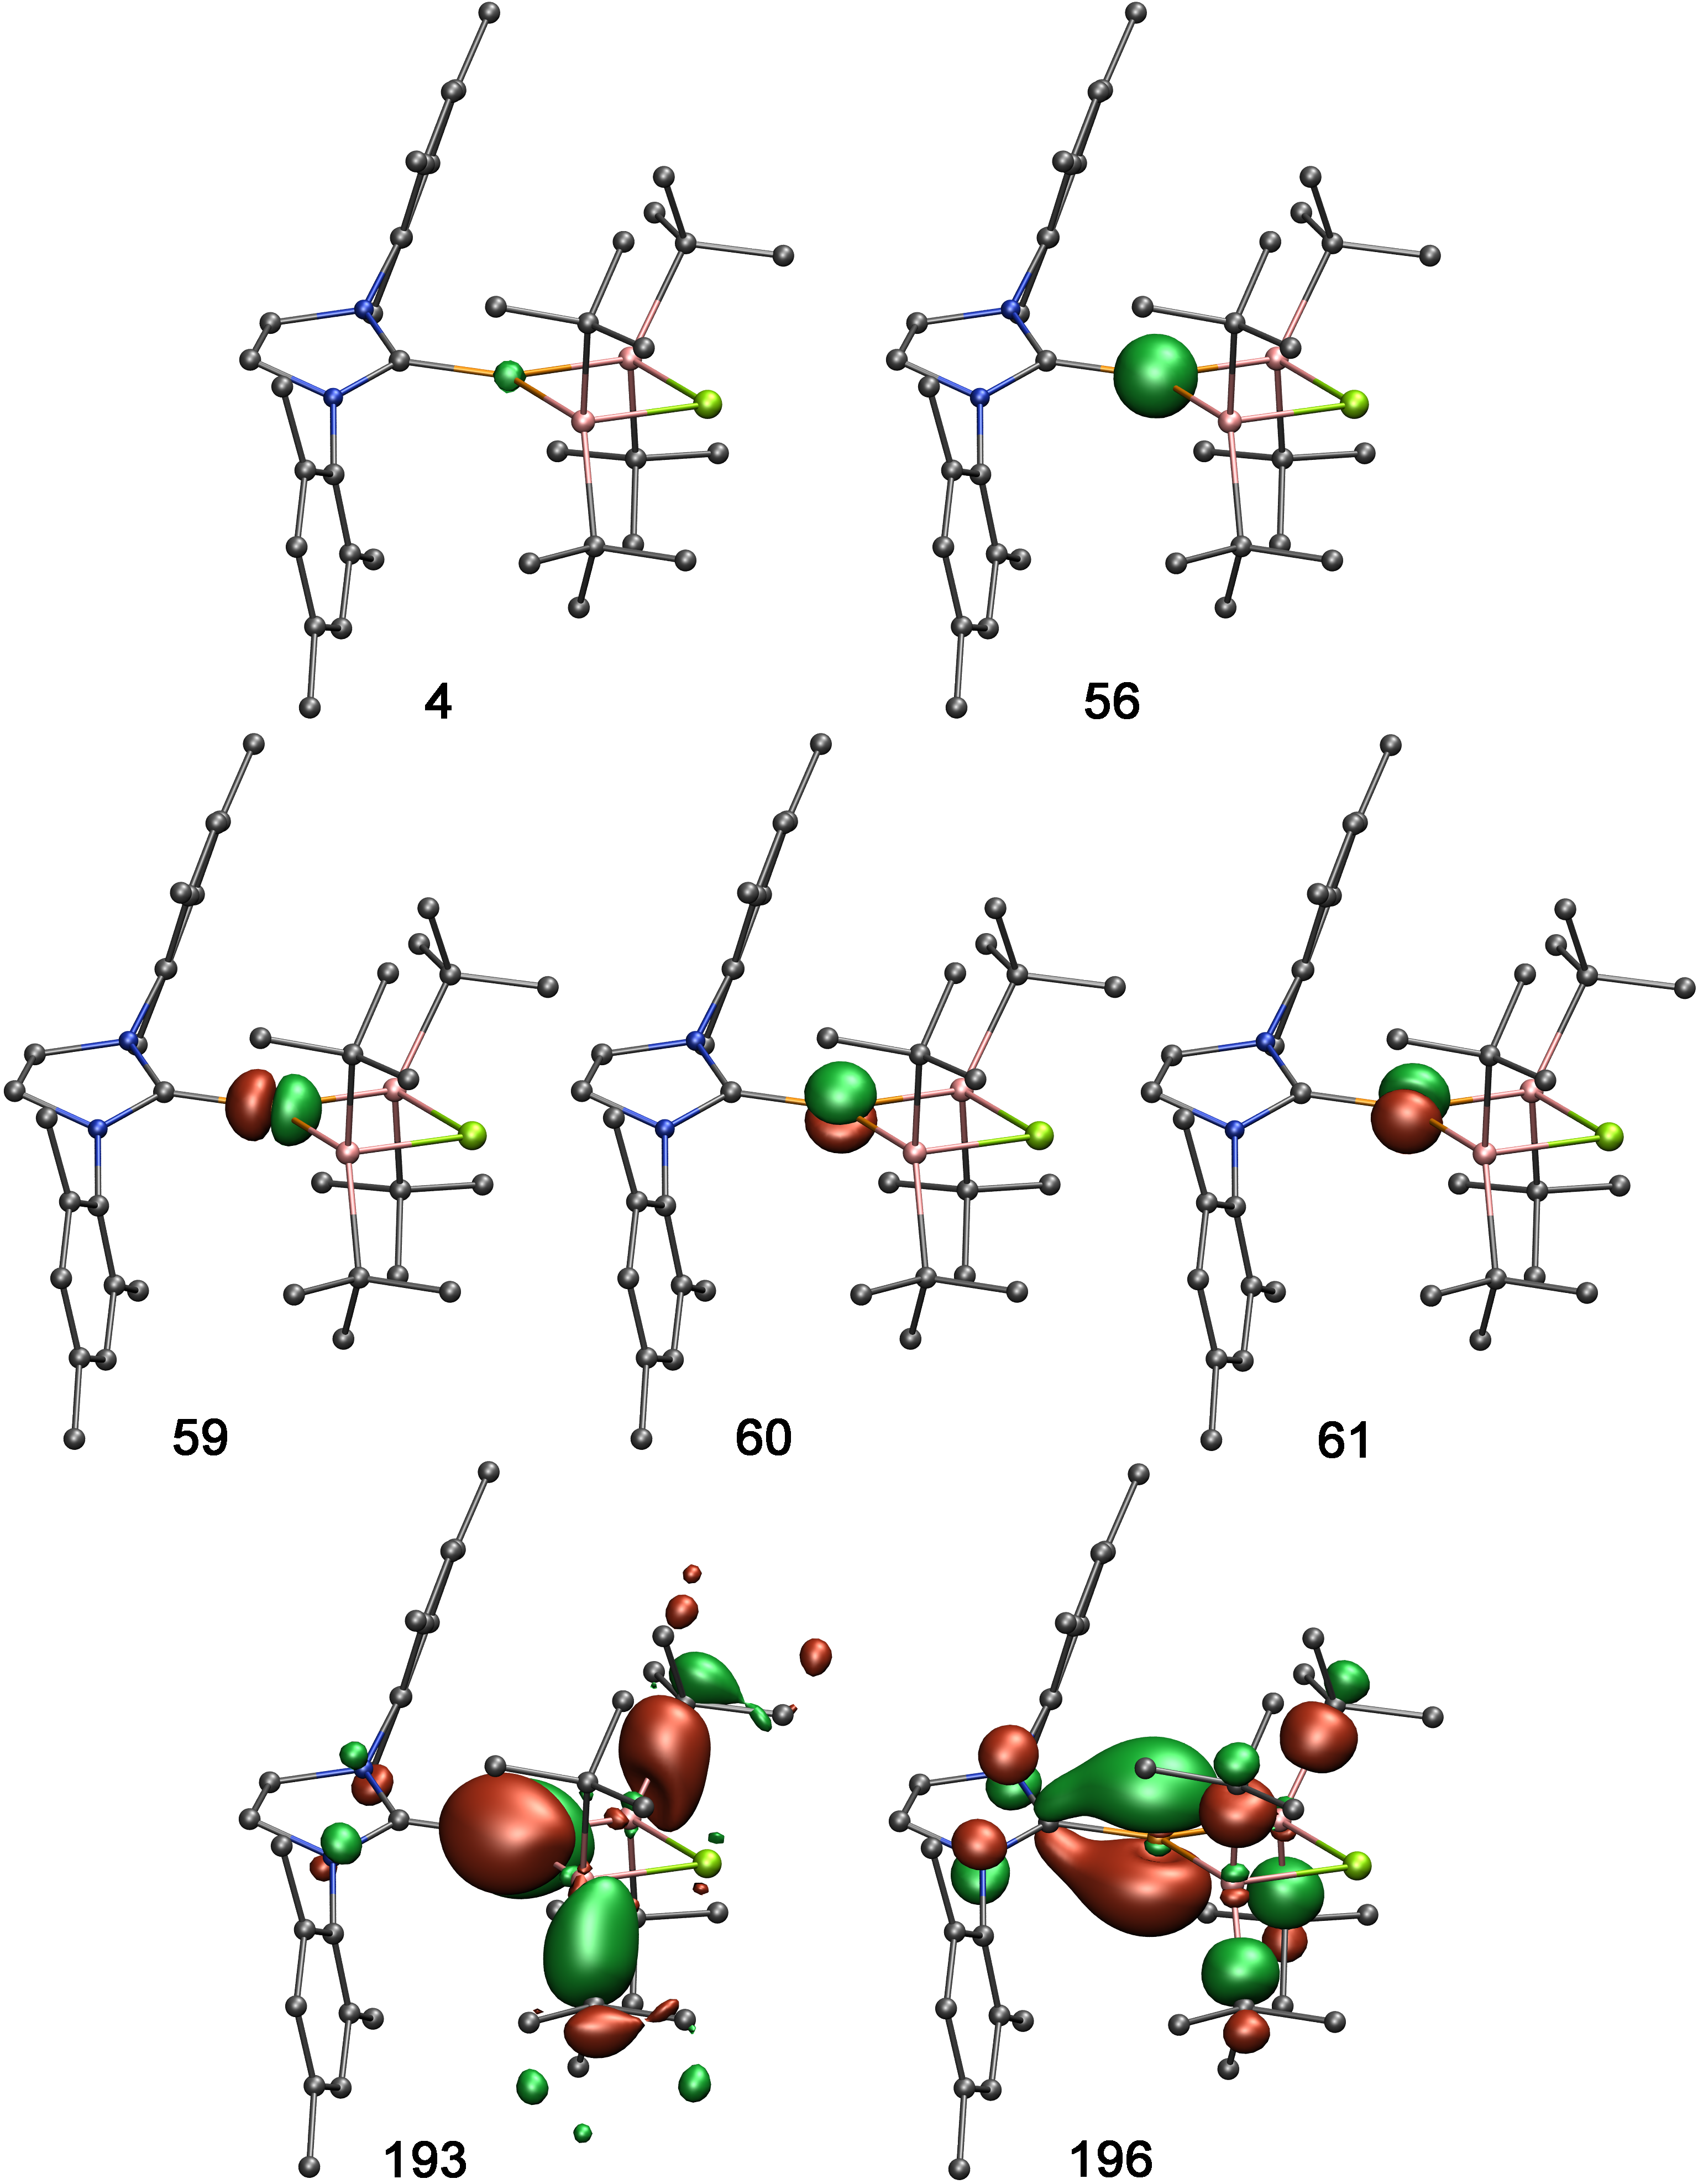
\includegraphics[width=0.80\textwidth]{modec}
	\captionsetup{figurewithin = chapter}
	\captionsetup{font=small, labelfont=bf}\caption[{Molekülorbitale von SIMesP(Ga$^\textit{t}$Bu$_2$)$_2$Cl}]{Molekülorbitale mit den größten Beiträgen zur $^{31}$P-Abschirmung in \mbox{SIMesP(Ga$^\textit{t}$Bu$_2$)$_2$Cl}. Im Einzelnen ist \textbf{\textsf{4}} das 1$s$-Orbital, \textbf{\textsf{56}} das 2$s$-Orbital und \textbf{\textsf{59}}--\textbf{\textsf{61}} sind die 2$p$-Orbitale des Phosphors. \textbf{\textsf{193}} und \textbf{\textsf{196}} sind die C--P-$\pi$-Orbitale. Gleichzeitig ist 196 auch das höchst besetzte \ac{mo} der Verbindung (Kohlenstoff=grau, Stickstoff=blau, Phosphor=orange, Gallium=rosa und Chlor=grün). Die Wasserstoffatome wurden zur besseren Veranschaulichung bei der Abbildung weggelassen.}
\label{abb:modec}
\end{figure}

{\footnotesize\begin{longtabu}to\textwidth{X[2,r]X[4,r]X[4,r]X[4,r]X[4,r]X[1,c]}
%{\footnotesize\begin{longtabu}to\textwidth{S[table-format = 3.0]S[table-format = 4.3]S[table-format = 3.8]S[table-format = 3.8]S[table-format = 3.8]X[1,c]}
\captionsetup{tablewithin = chapter}
\captionsetup{font=small, labelfont=bf}
\captionabove[{Zerlegung der $^{31}$P-chemischen Verschiebung in Orbitalbeiträge}]{\ac{mo}-Beiträge zur $^{31}$P-chemischen Verschiebung. Orbitale, die weniger als \unit[1]{ppm} beitragen, wurden nicht aufgenommen. Die am meisten beitragenden Orbitale wurden mit einem X gekennzeichnet und sind in Abbildung \ref{abb:modec} gezeigt. Zur Reduktion der Probleme, die durch die Eichinvarianz auftreten, wurde das Molekül so verschoben, dass das Phosphoratom im Ursprung liegt.\label{tab:cvhzerlegung}}\\
    \hline
    \hline
    \ac{mo} & \text{Energie} / \text{eV} & \text{diamagnetischer} & \text{paramagnetischer} & \text{gesamt} &  \\
     &  & \text{Beitrag\;\;\;\;\;\;\;\;} & \text{Beitrag\;\;\;\;\;\;\;\;} &  &  \\
    \hline
    %
  \endfirsthead % Erster Kopf zu Ende
  \multicolumn{6}{l}{\ldots\, \text{Fortsetzung}}\\
  \ac{mo} & \text{Energie} / \text{eV} & \text{diamagnetischer} & \text{paramagnetischer} & \text{gesamt} &  \\ 
   &  & \text{Beitrag\;\;\;\;\;\;\;\;} & \text{Beitrag\;\;\;\;\;\;\;\;} &  &  \\ 
  \hline
  \endhead
%
  \multicolumn{6}{r}{\text{wird fortgesetzt} \ldots}
  \endfoot
  \endlastfoot
%	\endfirsthead % Erster Kopf zu Ende
	%  Definition des Tabellenkopfes auf den folgenden Seiten
%	\caption{Fortsetzung}\\%
%	\ac{mo} & Energie / eV & diamagnetischer Beitrag & paramagnetischer Beitrag & gesamt &  \\
%	\hline
%	\endhead % Zweiter Kopf ist zu Ende
%	Weiter auf der n{\"a}chste Seite\\
%	\endfoot
%	\hline
%	Vor dem endlastfoot: Tabelle zu Ende \\
%\endlastfoot
% Ab hier kommt der Inhalt der Tabelle
%    4             & $\num{-2075.219}$ &$\num{517.191836}$ &$\num{-0.00453970}$ &$\num{517.187296}$ & X \\
%    56            & $\num{-170.577}$  &$\num{99.4654758}$ &$\num{0.09861722}$ &$\num{99.5640930}$ & X \\
%    59            & $\num{-122.029}$  &$\num{92.6938755}$ &$\num{34.7117998}$ &$\num{127.405675}$ & X \\
%    60            & $\num{-121.991}$  &$\num{95.9498071}$ &$\num{-4.87383336}$ &$\num{91.0759738}$ & X \\
%    61            & $\num{-121.983}$  &$\num{95.8039826}$ &$\num{-5.30359114}$ &$\num{90.5003915}$ & X \\
%    68            & $\num{-25.662}$   &$\num{0.53404716}$ &$\num{1.35462150}$ &$\num{1.88866866}$ &  \\
%    69            & $\num{-23.408}$   &$\num{-0.09814514}$ &$\num{3.16604807}$ &$\num{3.06790293}$ &  \\
%    70            & $\num{-21.627}$   &$\num{0.01959928}$ &$\num{1.78702756}$ &$\num{1.80662684}$ &  \\
%    71            & $\num{-21.234}$   &$\num{0.02197222}$ &$\num{1.95831192}$ &$\num{1.98028413}$ &  \\
%    72            & $\num{-19.775}$   &$\num{-0.01793399}$ &$\num{2.45924440}$ &$\num{2.44131041}$ &  \\
%    73            & $\num{-19.633}$   &$\num{0.24167534}$ &$\num{6.54078556}$ &$\num{6.78246089}$ &  \\
%    74            & $\num{-19.570}$   &$\num{-0.02172001}$ &$\num{1.09340645}$ &$\num{1.07168644}$ &  \\
%    76            & $\num{-19.473}$   &$\num{0.09386996}$ &$\num{2.11593358}$ &$\num{2.20980355}$ &  \\
%    77            & $\num{-19.446}$   &$\num{0.08714956}$ &$\num{1.87050869}$ &$\num{1.95765824}$ &  \\
%    78            & $\num{-19.368}$   &$\num{0.13194102}$ &$\num{2.12303904}$ &$\num{2.25498006}$ &  \\
%    79            & $\num{-19.362}$   &$\num{0.49287261}$ &$\num{-4.45535897}$ &$\num{-3.96248637}$ &  \\
%    80            & $\num{-19.357}$   &$\num{0.18579217}$ &$\num{1.20863043}$ &$\num{1.39442260}$ &  \\
%    81            & $\num{-19.202}$   &$\num{-0.00201103}$ &$\num{1.59801150}$ &$\num{1.59600048}$ &  \\
%    93            & $\num{-17.403}$   &$\num{0.01353283}$ &$\num{2.14047301}$ &$\num{2.15400584}$ &  \\
%    94            & $\num{-17.354}$   &$\num{-0.01692121}$ &$\num{1.55183281}$ &$\num{1.53491159}$ &  \\
%    95            & $\num{-16.901}$   &$\num{-0.01320885}$ &$\num{1.12779650}$ &$\num{1.11458766}$ &  \\
%    96            & $\num{-16.814}$   &$\num{0.01229753}$ &$\num{1.00358603}$ &$\num{1.01588356}$ &  \\
%    97            & $\num{-16.764}$   &$\num{-0.01172257}$ &$\num{1.21713482}$ &$\num{1.20541225}$ &  \\
%    98            & $\num{-16.437}$   &$\num{0.02021503}$ &$\num{1.63625805}$ &$\num{1.65647307}$ &  \\
%    99            & $\num{-16.434}$   &$\num{0.06779826}$ &$\num{1.45607779}$ &$\num{1.52387604}$ &  \\
%    100           & $\num{-16.374}$   &$\num{0.06596182}$ &$\num{1.75989832}$ &$\num{1.82586014}$ &  \\
%    101           & $\num{-16.303}$   &$\num{0.03007284}$ &$\num{1.32661045}$ &$\num{1.35668329}$ &  \\
%    102           & $\num{-16.290}$   &$\num{0.01787841}$ &$\num{1.52573046}$ &$\num{1.54360887}$ &  \\
%    103           & $\num{-16.268}$   &$\num{0.02568144}$ &$\num{1.42316584}$ &$\num{1.44884728}$ &  \\
%    104           & $\num{-16.195}$   &$\num{0.01887398}$ &$\num{1.47227302}$ &$\num{1.49114700}$ &  \\
%    105           & $\num{-16.142}$   &$\num{0.02095796}$ &$\num{1.50018399}$ &$\num{1.52114195}$ &  \\
%    106           & $\num{-15.952}$   &$\num{0.04972872}$ &$\num{1.53983104}$ &$\num{1.58955976}$ &  \\
%    107           & $\num{-15.680}$   &$\num{6.94363928}$ &$\num{0.69097726}$ &$\num{7.63461654}$ &  \\
%    108           & $\num{-15.051}$   &$\num{3.05882791}$ &$\num{2.36501176}$ &$\num{5.42383967}$ &  \\
%    112           & $\num{-13.518}$   &$\num{0.81685183}$ &$\num{0.74118574}$ &$\num{1.55803757}$ &  \\
%    113           & $\num{-13.116}$   &$\num{0.16457604}$ &$\num{1.78343911}$ &$\num{1.94801516}$ &  \\
%    114           & $\num{-12.945}$   &$\num{1.25055266}$ &$\num{-0.04451094}$ &$\num{1.20604171}$ &  \\
%    115           & $\num{-12.836}$   &$\num{0.16214427}$ &$\num{-1.90735225}$ &$\num{-1.74520798}$ &  \\
%    116           & $\num{-12.561}$   &$\num{0.14150550}$ &$\num{1.15076135}$ &$\num{1.29226684}$ &  \\
%    117           & $\num{-12.556}$   &$\num{3.78081903}$ &$\num{5.91381542}$ &$\num{9.69463445}$ &  \\
%    118           & $\num{-12.483}$   &$\num{0.12979966}$ &$\num{1.07317233}$ &$\num{1.20297198}$ &  \\
%    119           & $\num{-12.480}$   &$\num{0.32351403}$ &$\num{1.25053545}$ &$\num{1.57404948}$ &  \\
%    120           & $\num{-12.129}$   &$\num{0.54584208}$ &$\num{1.34398803}$ &$\num{ 1.88983012}$ &  \\
%    121           & $\num{-11.930}$   &$\num{0.09249229}$ &$\num{3.24272225}$ &$\num{3.33521454}$ &  \\
%    122           & $\num{-11.276}$   &$\num{0.44510731}$ &$\num{-16.7759414}$ &$\num{-16.3308341}$ &  \\
%    123           & $\num{-11.273}$   &$\num{0.33385082}$ &$\num{-9.09367970}$ &$\num{-8.75982889}$ &  \\
%    124           & $\num{-11.139}$   &$\num{0.17615005}$ &$\num{-1.64865544}$ &$\num{-1.47250539}$ &  \\
%    125           & $\num{-11.108}$   &$\num{0.51873119}$ &$\num{-5.03044193}$ &$\num{-4.51171074}$ &  \\
%    126           & $\num{-10.787}$   &$\num{0.03447635}$ &$\num{-1.21731750}$ &$\num{-1.18284116}$ &  \\
%    127           & $\num{-10.726}$   &$\num{0.06770143}$ &$\num{1.40499911}$ &$\num{1.47270054}$ &  \\
%    128           & $\num{-10.662}$   &$\num{0.06156794}$ &$\num{2.91941845}$ &$\num{2.98098640}$ &  \\
%    134           & $\num{-10.281}$   &$\num{0.04467939}$ &$\num{1.25376753}$ &$\num{1.29844691}$ &  \\
%    136           & $\num{-10.209}$   &$\num{0.48598321}$ &$\num{-9.11261675}$ &$\num{-8.62663355}$ &  \\
%    137           & $\num{-10.185}$   &$\num{0.07291205}$ &$\num{1.55274159}$ &$\num{1.62565365}$ &  \\
%    138           & $\num{-10.144}$   &$\num{0.07830575}$ &$\num{1.02481432}$ &$\num{1.10312007}$ &  \\
%    141           & $\num{-10.066}$   &$\num{0.13647590}$ &$\num{-1.83547857}$ &$\num{-1.69900267}$&  \\
%    143           & $\num{-9.962}$    &$\num{0.18119511}$ &$\num{-11.9269724}$ &$\num{-11.7457772}$&  \\
%    145           & $\num{-9.901}$    &$\num{0.54552586}$ &$\num{-6.83025033}$ &$\num{-6.28472447}$&  \\
%    146           & $\num{-9.893}$    &$\num{0.01054856}$ &$\num{1.15279966}$ &$\num{1.16334822}$&  \\
%    148           & $\num{-9.795}$    &$\num{0.04937586}$ &$\num{-1.11751888}$ &$\num{-1.06814303}$&  \\
%    149           & $\num{-9.771}$    &$\num{1.57970367}$ &$\num{-35.4394600}$ &$\num{-33.8597563}$&  \\
%    150           & $\num{-9.749}$    &$\num{1.05654025}$ &$\num{-36.5240686}$ &$\num{-35.4675283}$&  \\
%    151           & $\num{-9.616}$    &$\num{0.14242252}$ &$\num{-3.05971013}$ &$\num{-2.91728761}$&  \\
%    152           & $\num{-9.603}$    &$\num{0.54286829}$ &$\num{-14.0900846}$ &$\num{-13.5472163}$&  \\
%    154           & $\num{-9.078}$    &$\num{0.45679481}$ &$\num{-6.25269617}$ &$\num{-5.79590137}$&  \\
%    155           & $\num{-9.022}$    &$\num{0.30521796}$ &$\num{-2.89719583}$ &$\num{-2.59197787}$&  \\
%    157           & $\num{-8.915}$    &$\num{0.33176040}$ &$\num{-12.0465755}$ &$\num{-11.7148151}$&  \\
%    158           & $\num{-8.894}$    &$\num{0.03499415}$ &$\num{-2.23272019}$ &$\num{-2.19772604}$&  \\
%    159           & $\num{-8.852}$    &$\num{0.12790544}$ &$\num{-1.78054627}$ &$\num{-1.65264083}$&  \\
%    160           & $\num{-8.836}$    &$\num{0.11569778}$ &$\num{-4.18203675}$ &$\num{-4.06633897}$&  \\
%    161           & $\num{-8.821}$    &$\num{0.22141616}$ &$\num{-2.88978294}$ &$\num{-2.66836679}$&  \\
%    163           & $\num{-8.685}$    &$\num{-0.04341331}$ &$\num{-1.06858108}$ &$\num{-1.11199439}$&  \\
%    164           & $\num{-8.613}$    &$\num{-0.03929554}$ &$\num{-1.37310952}$ &$\num{-1.41240506}$&  \\
%    165           & $\num{-8.567}$    &$\num{0.49516778}$ &$\num{-14.9968916}$ &$\num{-14.5017238}$&  \\
%    166           & $\num{-8.416}$    &$\num{0.03588159}$ &$\num{-2.28427077}$ &$\num{-2.24838919}$&  \\
%    167           & $\num{-8.368}$    &$\num{0.00248013}$ &$\num{-2.06308801}$ &$\num{-2.06060789}$&  \\
%    168           & $\num{-8.331}$    &$\num{0.03514653}$ &$\num{-2.25281836}$ &$\num{-2.21767183}$&  \\
%    169           & $\num{-8.325}$    &$\num{0.03804272}$ &$\num{-1.08383300}$ &$\num{-1.04579028}$&  \\
%    170           & $\num{-8.287}$    &$\num{0.01021177}$ &$\num{-2.13399407}$ &$\num{-2.12378230}$&  \\
%    171           & $\num{-8.262}$    &$\num{-0.01101696}$ &$\num{-1.80433784}$ &$\num{-1.81535480}$&  \\
%    172           & $\num{-8.251}$    &$\num{0.03656101}$ &$\num{-2.51568170}$ &$\num{-2.47912069}$&  \\
%    173           & $\num{-8.164}$    &$\num{0.03218817}$ &$\num{-1.95963980}$ &$\num{-1.92745163}$&  \\
%    174           & $\num{-8.159}$    &$\num{0.01339373}$ &$\num{-1.20803182}$ &$\num{-1.19463810}$&  \\
%    175           & $\num{-8.024}$    &$\num{0.27091016}$ &$\num{-4.46817721}$ &$\num{-4.19726705}$&  \\
%    176           & $\num{-7.651}$    &$\num{0.16272505}$ &$\num{-5.41820816}$ &$\num{-5.25548311}$&  \\
%    177           & $\num{-7.511}$    &$\num{0.58622111}$ &$\num{-28.1015327}$ &$\num{-27.5153116}$&  \\
%    178           & $\num{-7.498}$    &$\num{0.06000340}$ &$\num{-2.75059261}$ &$\num{-2.69058921}$&  \\
%    179           & $\num{-7.436}$    &$\num{0.03258139}$ &$\num{-3.88194160}$ &$\num{-3.84936020}$&  \\
%    180           & $\num{-7.357}$    &$\num{0.04926782}$ &$\num{-3.68748232}$ &$\num{-3.63821451}$&  \\
%    181           & $\num{-7.310}$    &$\num{1.39166476}$ &$\num{-39.4294645}$ &$\num{-38.0377997}$&  \\
%    182           & $\num{-7.282}$    &$\num{0.04584765}$ &$\num{-2.46897227}$ &$\num{-2.42312462}$&  \\
%    183           & $\num{-7.154}$    &$\num{1.64417751}$ &$\num{-46.0412125}$ &$\num{-44.3970350}$&  \\
%    184           & $\num{-7.140}$    &$\num{0.81407613}$ &$\num{-24.8477059}$ &$\num{-24.0336297}$&  \\
%    185           & $\num{-6.995}$    &$\num{1.21851146}$ &$\num{-33.2754464}$ &$\num{-32.0569350}$&  \\
%    186           & $\num{-6.930}$    &$\num{1.92326147}$ &$\num{-41.6456079}$ &$\num{-39.7223464}$&  \\
%    187           & $\num{-6.520}$    &$\num{0.96541333}$ &$\num{2.86932743}$ &$\num{3.83474076}$&  \\
%    188           & $\num{-6.399}$    &$\num{0.13594597}$ &$\num{1.04337865}$ &$\num{1.17932463}$&  \\
%    189           & $\num{-6.079}$    &$\num{0.38325442}$ &$\num{-10.3976843}$ &$\num{-10.0144298}$&  \\
%    191           & $\num{-6.027}$    &$\num{0.02032565}$ &$\num{-3.14864368}$ &$\num{-3.12831803}$&  \\
%    192           & $\num{-5.516}$    &$\num{0.19730284}$ &$\num{-22.6888381}$ &$\num{-22.4915353}$&  \\
%    193           & $\num{-5.214}$    &$\num{7.32158116}$ &$\num{-75.1069516}$ &$\num{-67.7853704}$& X \\
%    194           & $\num{-5.099}$    &$\num{6.68651778}$ &$\num{4.86354126}$ &$\num{11.5500590}$&  \\
%    195           & $\num{-4.892}$    &$\num{0.15622881}$ &$\num{-4.87733749}$ &$\num{-4.72110868}$&  \\
%    196           & $\num{-4.434}$    &$\num{7.95638357}$ &$\num{-117.389691}$ &$\num{-109.433307}$& X \\
%    \text{gesamt} &                   &$\num{962.655788}$ &$\num{-581.846494}$ &$\num{380.809294}$&  \\
    4     & $-$2075.219 & 517.191836 & $-$0.00453970 & 517.187296 & X \\
    56    & $-$170.577  & 99.4654758 &  0.09861722 & 99.5640930 & X \\
    59    & $-$122.029  & 92.6938755 &  34.7117998 & 127.405675 & X \\
    60    & $-$121.991  & 95.9498071 & $-$4.87383336 & 91.0759738 & X \\
    61    & $-$121.983  & 95.8039826 & $-$5.30359114 & 90.5003915 & X \\
    68    & $-$25.662 & 0.53404716 & 1.35462150 & 1.88866866 &  \\
    69    & $-$23.408 &$-$0.09814514 & 3.16604807 & 3.06790293 &  \\
    70    & $-$21.627 & 0.01959928 & 1.78702756 & 1.80662684 &  \\
    71    & $-$21.234 & 0.02197222 & 1.95831192 & 1.98028413 &  \\
    72    & $-$19.775 &$-$0.01793399 & 2.45924440 & 2.44131041 &  \\
    73    & $-$19.633 & 0.24167534 & 6.54078556 & 6.78246089 &  \\
    74    & $-$19.570 &$-$0.02172001 & 1.09340645 & 1.07168644 &  \\
    76    & $-$19.473 & 0.09386996 & 2.11593358 & 2.20980355 &  \\
    77    & $-$19.446 & 0.08714956 & 1.87050869 & 1.95765824 &  \\
    78    & $-$19.368 & 0.13194102 & 2.12303904 & 2.25498006 &  \\
    79    & $-$19.362 & 0.49287261 &$-$4.45535897 &$-$3.96248637 &  \\
    80    & $-$19.357 & 0.18579217 & 1.20863043 & 1.39442260 &  \\
    81    & $-$19.202 &$-$0.00201103 & 1.59801150 & 1.59600048 &  \\
    93    & $-$17.403 & 0.01353283 & 2.14047301 & 2.15400584 &  \\
    94    & $-$17.354 &$-$0.01692121 & 1.55183281 & 1.53491159 &  \\
    95    & $-$16.901 &$-$0.01320885 & 1.12779650 & 1.11458766 &  \\
    96    & $-$16.814 & 0.01229753 & 1.00358603 & 1.01588356 &  \\
    97    & $-$16.764 &$-$0.01172257 & 1.21713482 & 1.20541225 &  \\
    98    & $-$16.437 & 0.02021503 & 1.63625805 & 1.65647307 &  \\
    99    & $-$16.434 & 0.06779826 & 1.45607779 & 1.52387604 &  \\
    100   & $-$16.374 & 0.06596182 & 1.75989832 & 1.82586014 &  \\
    101   & $-$16.303 & 0.03007284 & 1.32661045 & 1.35668329 &  \\
    102   & $-$16.290 & 0.01787841 & 1.52573046 & 1.54360887 &  \\
    103   & $-$16.268 & 0.02568144 & 1.42316584 & 1.44884728 &  \\
    104   & $-$16.195 & 0.01887398 & 1.47227302 & 1.49114700 &  \\
    105   & $-$16.142 & 0.02095796 & 1.50018399 & 1.52114195 &  \\
    106   & $-$15.952 & 0.04972872 & 1.53983104 & 1.58955976 &  \\
    107   & $-$15.680 & 6.94363928 & 0.69097726 & 7.63461654 &  \\
    108   & $-$15.051 & 3.05882791 & 2.36501176 & 5.42383967 &  \\
    112   & $-$13.518 & 0.81685183 & 0.74118574 & 1.55803757 &  \\
    113   & $-$13.116 & 0.16457604 & 1.78343911 & 1.94801516 &  \\
    114   & $-$12.945 & 1.25055266 &$-$0.04451094 & 1.20604171 &  \\
    115   & $-$12.836 & 0.16214427 &$-$1.90735225 &$-$1.74520798 &  \\
    116   & $-$12.561 & 0.14150550 & 1.15076135 & 1.29226684 &  \\
    117   & $-$12.556 & 3.78081903 & 5.91381542 & 9.69463445 &  \\
    118   & $-$12.483 & 0.12979966 & 1.07317233 & 1.20297198 &  \\
    119   & $-$12.480 & 0.32351403 & 1.25053545 & 1.57404948 &  \\
    120   & $-$12.129 & 0.54584208 & 1.34398803 & 1.88983012 &  \\
    121   & $-$11.930 & 0.09249229 & 3.24272225 & 3.33521454 &  \\
    122   & $-$11.276 & 0.44510731 &$-$16.7759414 &$-$16.3308341 &  \\
    123   & $-$11.273 & 0.33385082 &$-$9.09367970 &$-$8.75982889 &  \\
    124   & $-$11.139 & 0.17615005 &$-$1.64865544 &$-$1.47250539 &  \\
    125   & $-$11.108 & 0.51873119 &$-$5.03044193 &$-$4.51171074 &  \\
    126   & $-$10.787 & 0.03447635 &$-$1.21731750 &$-$1.18284116 &  \\
    127   & $-$10.726 & 0.06770143 & 1.40499911 & 1.47270054 &  \\
    128   & $-$10.662 & 0.06156794 & 2.91941845 & 2.98098640 &  \\
    134   & $-$10.281 & 0.04467939 & 1.25376753 & 1.29844691 &  \\
    136   & $-$10.209 & 0.48598321 &$-$9.11261675 &$-$8.62663355 &  \\
    137   & $-$10.185 & 0.07291205 & 1.55274159 & 1.62565365 &  \\
    138   & $-$10.144 & 0.07830575 & 1.02481432 & 1.10312007 &  \\
    141   & $-$10.066 & 0.13647590 &$-$1.83547857 & $-$1.69900267 &  \\
    143   & $-$9.962 & 0.18119511 & $-$11.9269724 & $-$11.7457772 &  \\
    145   & $-$9.901 & 0.54552586 & $-$6.83025033 & $-$6.28472447 &  \\
    146   & $-$9.893 & 0.01054856 &  1.15279966 &  1.16334822 &  \\
    148   & $-$9.795 & 0.04937586 & $-$1.11751888 & $-$1.06814303 &  \\
    149   & $-$9.771 & 1.57970367 & $-$35.4394600 & $-$33.8597563 &  \\
    150   & $-$9.749 & 1.05654025 & $-$36.5240686 & $-$35.4675283 &  \\
    151   & $-$9.616 & 0.14242252 & $-$3.05971013 & $-$2.91728761 &  \\
    152   & $-$9.603 & 0.54286829 & $-$14.0900846 & $-$13.5472163 &  \\
    154   & $-$9.078 & 0.45679481 & $-$6.25269617 & $-$5.79590137 &  \\
    155   & $-$9.022 & 0.30521796 & $-$2.89719583 & $-$2.59197787 &  \\
    157   & $-$8.915 & 0.33176040 & $-$12.0465755 & $-$11.7148151 &  \\
    158   & $-$8.894 & 0.03499415 & $-$2.23272019 & $-$2.19772604 &  \\
    159   & $-$8.852 & 0.12790544 & $-$1.78054627 & $-$1.65264083 &  \\
    160   & $-$8.836 & 0.11569778 & $-$4.18203675 & $-$4.06633897 &  \\
    161   & $-$8.821 & 0.22141616 & $-$2.88978294 & $-$2.66836679 &  \\
    163   & $-$8.685 &$-$0.04341331 & $-$1.06858108 & $-$1.11199439 &  \\
    164   & $-$8.613 &$-$0.03929554 & $-$1.37310952 & $-$1.41240506 &  \\
    165   & $-$8.567 & 0.49516778 & $-$14.9968916 & $-$14.5017238 &  \\
    166   & $-$8.416 & 0.03588159 & $-$2.28427077 & $-$2.24838919 &  \\
    167   & $-$8.368 & 0.00248013 & $-$2.06308801 & $-$2.06060789 &  \\
    168   & $-$8.331 & 0.03514653 & $-$2.25281836 & $-$2.21767183 &  \\
    169   & $-$8.325 & 0.03804272 & $-$1.08383300 & $-$1.04579028 &  \\
    170   & $-$8.287 & 0.01021177 & $-$2.13399407 & $-$2.12378230 &  \\
    171   & $-$8.262 &$-$0.01101696 & $-$1.80433784 & $-$1.81535480 &  \\
    172   & $-$8.251 & 0.03656101 & $-$2.51568170 & $-$2.47912069 &  \\
    173   & $-$8.164 & 0.03218817 & $-$1.95963980 & $-$1.92745163 &  \\
    174   & $-$8.159 & 0.01339373 & $-$1.20803182 & $-$1.19463810 &  \\
    175   & $-$8.024 & 0.27091016 & $-$4.46817721 & $-$4.19726705 &  \\
    176   & $-$7.651 & 0.16272505 & $-$5.41820816 & $-$5.25548311 &  \\
    177   & $-$7.511 & 0.58622111 & $-$28.1015327 & $-$27.5153116 &  \\
    178   & $-$7.498 & 0.06000340 & $-$2.75059261 & $-$2.69058921 &  \\
    179   & $-$7.436 & 0.03258139 & $-$3.88194160 & $-$3.84936020 &  \\
    180   & $-$7.357 & 0.04926782 & $-$3.68748232 & $-$3.63821451 &  \\
    181   & $-$7.310 & 1.39166476 & $-$39.4294645 & $-$38.0377997 &  \\
    182   & $-$7.282 & 0.04584765 & $-$2.46897227 & $-$2.42312462 &  \\
    183   & $-$7.154 & 1.64417751 & $-$46.0412125 & $-$44.3970350 &  \\
    184   & $-$7.140 & 0.81407613 & $-$24.8477059 & $-$24.0336297 &  \\
    185   & $-$6.995 & 1.21851146 & $-$33.2754464 & $-$32.0569350 &  \\
    186   & $-$6.930 & 1.92326147 & $-$41.6456079 & $-$39.7223464 &  \\
    187   & $-$6.520 & 0.96541333 &  2.86932743 &  3.83474076 &  \\
    188   & $-$6.399 & 0.13594597 &  1.04337865 &  1.17932463 &  \\
    189   & $-$6.079 & 0.38325442 & $-$10.3976843 & $-$10.0144298 &  \\
    191   & $-$6.027 & 0.02032565 & $-$3.14864368 & $-$3.12831803 &  \\
    192   & $-$5.516 & 0.19730284 & $-$22.6888381 & $-$22.4915353 &  \\
    193   & $-$5.214 & 7.32158116 & $-$75.1069516 & $-$67.7853704 & X \\
    194   & $-$5.099 & 6.68651778 &  4.86354126 &  11.5500590 &  \\
    195   & $-$4.892 & 0.15622881 & $-$4.87733749 & $-$4.72110868 &  \\
    196   & $-$4.434 & 7.95638357 & $-$117.389691 & $-$109.433307 & X \\
    \text{gesamt} &       & 962.655788 & $-$581.846494 &  380.809294 &  \\
\end{longtabu}}%

\begin{table}[ht!]
  	\centering
	\captionsetup{tablewithin = chapter}
	\captionsetup{font=small, labelfont=bf}
	\captionabove[Absolute chemische Abschirmungskonstanten mit \ac{cosmo}]{Absolute chemische Abschirmungskonstanten mit TPSSh/def2-TZVP und \ac{cosmo} für einen Testsatz organischer Moleküle aus Referenz \cite{fulmer2010nmr}. Das \ac{cosmo} wurde sowohl für die Optimierung der Strukturparameter als auch für die Berechnung der chemischen Abschirmungskonstanten verwendet.} 
	\resizebox{\textwidth}{!}{%
    \begin{tabular}{lrrrrrrrrrrrr}
    \hline
    \hline
    Molekül & THF-d$_{8}$ & CD$_{2}$Cl$_{2}$ & CDCl$_{3}$ & Toluol-d$_{8}$ & C$_{6}$D$_{6}$ & C$_{6}$D$_{5}$Cl & (CD$_{3}$)$_{2}$CO & (CD$_{3}$)$_{2}$SO & CD$_{3}$CN & TFE-d$_{3}$ & CD$_{3}$OD & D$_{2}$O\\
    \hline
	1,2-Dichlorethan & 136.24 & 136.20 & 136.39 & 136.68 & 136.69 & 136.33 & 136.05 & 135.97 & 135.99 & 136.21 & 136.00 & 135.95 \\
    1,4-Dioxan & 115.85 & 115.84 & 115.89 & 115.98 & 115.98 & 115.87 & 115.79 & 115.76 & 115.77 & 115.84 & 115.77 & 115.75 \\
    18-Krone-6 & 111.84 & 111.85 & 111.81 & 111.72 & 111.71 & 111.82 & 111.88 & 111.87 & 111.87 & 111.85 & 111.87 & 111.88 \\
    Aceton CH3 & 156.24 & 156.21 & 156.33 & 156.55 & 156.56 & 156.30 & 156.10 & 156.05 & 156.06 & 156.22 & 156.07 & 156.04 \\
    Aceton CO & $-$33.06 & $-$33.51 & $-$31.50 & $-$27.97 & $-$27.71 & $-$32.10 & $-$35.09 & $-$35.80 & $-$35.66 & $-$33.40 & $-$35.55 & $-$36.04 \\
    Acetonitril CH3 & 185.17 & 185.20 & 185.06 & 184.79 & 184.77 & 185.10 & 185.31 & 185.35 & 185.34 & 185.20 & 185.34 & 185.37 \\
    Acetonitril CN & 63.74 & 63.43 & 64.81 & 67.20 & 67.37 & 64.40 & 62.37 & 61.88 & 61.98 & 63.51 & 62.05 & 61.72 \\
    Benzol & 57.37 & 57.35 & 57.47 & 57.69 & 57.70 & 57.43 & 57.25 & 57.21 & 57.22 & 57.35 & 57.23 & 57.20 \\
    Chloroform & 79.23 & 79.19 & 79.38 & 79.73 & 79.76 & 79.34 & 79.03 & 78.95 & 78.96 & 79.20 & 78.98 & 78.93 \\
    Cyclohexan & 156.72 & 156.73 & 156.68 & 156.57 & 156.55 & 156.70 & 156.77 & 156.79 & 156.79 & 156.73 & 156.79 & 156.80 \\
    Dichlormethan & 114.90 & 114.81 & 115.20 & 115.84 & 115.88 & 115.09 & 114.50 & 114.35 & 114.38 & 114.84 & 114.40 & 114.30 \\
    Diethylether CH2 & 115.31 & 115.31 & 115.34 & 115.39 & 115.39 & 115.33 & 115.28 & 115.27 & 115.27 & 115.31 & 115.27 & 115.26 \\
    Diethylether CH3 & 170.06 & 170.09 & 169.99 & 169.81 & 169.79 & 170.02 & 170.15 & 170.18 & 170.18 & 170.08 & 170.17 & 170.19 \\
    Diglyme CH2\_1 & 111.77 & 111.77 & 111.77 & 111.76 & 111.76 & 111.77 & 111.78 & 111.77 & 111.77 & 111.77 & 111.78 & 111.77 \\
    Diglyme CH2\_2 & 110.50 & 110.50 & 110.48 & 110.43 & 110.43 & 110.49 & 110.52 & 110.53 & 110.52 & 110.50 & 110.52 & 110.53 \\
    Diglyme CH3 & 125.77 & 125.76 & 125.83 & 125.93 & 125.94 & 125.81 & 125.70 & 125.67 & 125.68 & 125.76 & 125.68 & 125.66 \\
    Dimethylformamid CH & 23.85 & 23.71 & 24.36 & 25.56 & 25.66 & 24.17 & 23.23 & 23.02 & 23.06 & 23.74 & 23.09 & 22.95 \\
    Dimethylformamid CH3\_1 & 156.28 & 156.27 & 156.29 & 156.30 & 156.31 & 156.29 & 156.25 & 156.24 & 156.24 & 156.27 & 156.24 & 156.24 \\
    Dimethylformamid CH3\_2 & 149.18 & 149.14 & 149.33 & 149.64 & 149.67 & 149.28 & 148.97 & 148.89 & 148.90 & 149.15 & 148.92 & 148.86 \\
    Essigsäure CH3 & 167.52 & 167.50 & 167.58 & 167.69 & 167.70 & 167.55 & 167.44 & 167.41 & 167.41 & 167.50 & 167.42 & 167.40 \\
    Essigsäure CO & 8.62  & 8.42  & 9.32  & 10.86 & 10.98 & 9.05  & 7.77  & 7.46  & 7.52  & 8.47  & 7.57  & 7.36 \\
    Ethan & 177.40 & 177.43 & 177.32 & 177.12 & 177.10 & 177.35 & 177.50 & 177.54 & 177.53 & 177.42 & 177.53 & 177.55 \\
    Ethanol CH2 & 122.69 & 122.68 & 122.74 & 122.83 & 122.84 & 122.73 & 122.63 & 122.60 & 122.61 & 122.68 & 122.61 & 122.59 \\
    Ethanol CH3 & 169.47 & 169.49 & 169.39 & 169.19 & 169.18 & 169.42 & 169.56 & 169.59 & 169.59 & 169.48 & 169.58 & 169.60 \\
    Ethen & 61.76 & 61.72 & 61.89 & 62.20 & 62.23 & 61.84 & 61.60 & 61.54 & 61.55 & 61.73 & 61.56 & 61.52 \\
    Ethylacetat CH2 & 119.99 & 119.92 & 120.21 & 120.71 & 120.75 & 120.13 & 119.69 & 119.59 & 119.61 & 119.94 & 119.63 & 119.56 \\
    Ethylacetat CH3 & 172.13 & 172.15 & 172.05 & 171.84 & 171.82 & 172.08 & 172.23 & 172.26 & 172.25 & 172.15 & 172.25 & 172.27 \\
    Ethylacetat CH3CO & 165.81 & 165.80 & 165.86 & 165.94 & 165.95 & 165.84 & 165.74 & 165.73 & 165.73 & 165.80 & 165.73 & 165.72 \\
    Ethylacetat CO & 8.77  & 8.60  & 9.43  & 10.86 & 10.96 & 9.18  & 7.97  & 7.70  & 7.75  & 8.65  & 7.79  & 7.59 \\
    Ethylenglycol & 118.45 & 118.44 & 118.45 & 118.42 & 118.41 & 118.44 & 118.42 & 118.41 & 118.42 & 118.44 & 118.42 & 118.41 \\
    Kohlenstoffdioxid & 59.89 & 59.89 & 59.89 & 59.91 & 59.92 & 59.89 & 59.88 & 59.87 & 59.87 & 59.89 & 59.87 & 59.87 \\
    Kohlenstoffdisulfid & $-$11.91 & $-$11.94 & $-$11.81 & $-$11.55 & $-$11.53 & $-$11.85 & $-$12.04 & $-$12.08 & $-$12.07 & $-$11.94 & $-$12.07 & $-$12.10 \\
    Methan & 192.54 & 192.57 & 192.41 & 192.11 & 192.09 & 192.46 & 192.69 & 192.74 & 192.73 & 192.56 & 192.72 & 192.76 \\
    Methanol & 132.34 & 132.32 & 132.40 & 132.50 & 132.50 & 132.38 & 132.26 & 132.23 & 132.24 & 132.33 & 132.24 & 132.22 \\
    n-Hexane CH2 (2,5) & 158.20 & 158.21 & 158.15 & 158.03 & 158.02 & 158.17 & 158.26 & 158.28 & 158.28 & 158.21 & 158.27 & 158.29 \\
    n-Hexane CH2 (3,4) & 149.36 & 149.37 & 149.32 & 149.22 & 149.21 & 149.33 & 149.41 & 149.43 & 149.42 & 149.37 & 149.42 & 149.43 \\
    n-Hexane CH3 & 170.35 & 170.37 & 170.27 & 170.09 & 170.07 & 170.30 & 170.44 & 170.47 & 170.46 & 170.36 & 170.46 & 170.48 \\
    Nitromethan & 122.68 & 122.62 & 122.88 & 123.32 & 123.35 & 122.81 & 122.41 & 122.32 & 122.34 & 122.64 & 122.35 & 122.28 \\
    n-Pentan CH2 (2,4) & 158.17 & 158.19 & 158.12 & 158.00 & 157.99 & 158.14 & 158.24 & 158.26 & 158.25 & 158.19 & 158.25 & 158.27 \\
    n-Pentan CH3 & 170.33 & 170.35 & 170.26 & 170.07 & 170.05 & 170.29 & 170.42 & 170.46 & 170.45 & 170.35 & 170.44 & 170.47 \\
    n-Pentane CH2 (3)  & 148.01 & 148.02 & 147.97 & 147.88 & 147.87 & 147.99 & 148.06 & 148.08 & 148.07 & 148.02 & 148.07 & 148.08 \\
    Propan CH2 & 165.40 & 165.42 & 165.35 & 165.22 & 165.21 & 165.37 & 165.47 & 165.49 & 165.49 & 165.41 & 165.48 & 165.50 \\
    Propan CH3 & 169.14 & 169.16 & 169.06 & 168.88 & 168.86 & 169.09 & 169.23 & 169.26 & 169.25 & 169.15 & 169.25 & 169.27 \\
    Propen CH & 48.09 & 47.99 & 46.42 & 47.21 & 47.27 & 48.29 & 47.66 & 47.52 & 47.54 & 48.01 & 47.57 & 47.47 \\
    Propen CH2 & 68.59 & 68.61 & 71.55 & 71.30 & 71.29 & 68.54 & 68.70 & 68.74 & 68.73 & 68.61 & 68.72 & 68.75 \\
    Propen CH3 & 170.88 & 170.89 & 164.60 & 164.46 & 164.45 & 170.85 & 170.94 & 170.96 & 170.95 & 170.89 & 170.95 & 170.96 \\
    Pyridin CH (2,6) & 34.73 & 34.72 & 34.77 & 34.88 & 34.89 & 34.76 & 34.70 & 34.70 & 34.70 & 34.72 & 34.70 & 34.70 \\
    Pyridin CH (3,5) & 62.33 & 62.25 & 62.60 & 63.14 & 63.17 & 62.50 & 61.99 & 61.87 & 61.89 & 62.27 & 61.91 & 61.83 \\
    Pyridin CH (4) & 49.41 & 49.30 & 49.81 & 50.62 & 50.67 & 49.67 & 48.91 & 48.73 & 48.77 & 49.33 & 48.79 & 48.67 \\
    Pyrrol CH (2,6) & 69.85 & 69.77 & 70.12 & 70.70 & 70.74 & 70.01 & 69.50 & 69.38 & 69.40 & 69.79 & 69.42 & 69.33 \\
    Pyrrol CH (3,4) & 79.61 & 79.68 & 79.36 & 78.84 & 78.80 & 79.45 & 79.94 & 80.07 & 80.04 & 79.66 & 80.02 & 80.11 \\
    Pyrrolidin CH2 (2,5) & 135.64 & 135.64 & 135.64 & 135.64 & 135.64 & 135.65 & 135.64 & 135.64 & 135.64 & 135.64 & 135.64 & 135.63 \\
    Pyrrolidin CH2 (3,4) & 160.93 & 160.94 & 160.88 & 160.78 & 160.77 & 160.90 & 160.98 & 160.99 & 160.99 & 160.93 & 160.99 & 161.00 \\
    Tetrachlormethan & 44.85 & 44.86 & 44.80 & 44.69 & 44.68 & 44.82 & 44.91 & 44.93 & 44.92 & 44.86 & 44.92 & 44.93 \\
    Toluol C (1) & 44.57 & 44.50 & 44.82 & 45.41 & 45.45 & 44.72 & 44.27 & 44.17 & 44.19 & 44.52 & 44.20 & 44.13 \\
    Toluol CH (2,6) & 56.76 & 56.74 & 56.83 & 56.99 & 57.00 & 56.80 & 56.67 & 56.64 & 56.64 & 56.74 & 56.65 & 56.63 \\
    Toluol CH (3,5) & 57.70 & 57.68 & 57.77 & 57.93 & 57.94 & 57.74 & 57.61 & 57.57 & 57.58 & 57.68 & 57.58 & 57.56 \\
    Toluol CH (4) & 60.77 & 60.76 & 60.80 & 60.87 & 60.87 & 60.79 & 60.73 & 60.72 & 60.72 & 60.77 & 60.72 & 60.71 \\
    Toluol CH3 & 163.74 & 163.76 & 163.68 & 163.52 & 163.50 & 163.70 & 163.84 & 163.86 & 163.86 & 163.76 & 163.85 & 163.88 \\
    Triethylamin CH2 & 135.95 & 135.96 & 135.95 & 135.97 & 135.97 & 135.95 & 135.95 & 135.96 & 135.96 & 135.96 & 135.95 & 135.95 \\
    Triethylamin CH3 & 171.50 & 171.51 & 171.43 & 171.28 & 171.27 & 171.46 & 171.57 & 171.59 & 171.58 & 171.51 & 171.58 & 171.60 \\
    \end{tabular}}%
  \label{tab:sigmacosmo}%
\end{table}%

\begin{table}[ht!]
  	\centering
	\captionsetup{tablewithin = chapter}
	\captionsetup{font=small, labelfont=bf}
	\captionabove[Absolute chemische Abschirmungskonstanten mit \ac{dcosmors}]{Absolute chemische Abschirmungskonstanten mit TPSSh/def2-TZVP und \ac{dcosmors} für einen Testsatz organischer Moleküle aus Referenz \cite{fulmer2010nmr}. Das \ac{dcosmors} wurde sowohl für die Optimierung der Strukturparameter als auch für die Berechnung der chemischen Abschirmungskonstanten verwendet.} 
	\resizebox{\textwidth}{!}{%
    \begin{tabular}{lrrrrrrrrrrrr}
    \hline
    \hline
    Molekül & THF-d$_{8}$ & CD$_{2}$Cl$_{2}$ & CDCl$_{3}$ & Toluol-d$_{8}$ & C$_{6}$D$_{6}$ & C$_{6}$D$_{5}$Cl & (CD$_{3}$)$_{2}$CO & (CD$_{3}$)$_{2}$SO & CD$_{3}$CN & TFE-d$_{3}$ & CD$_{3}$OD & D$_{2}$O\\
    \hline
    1,2-Dichlorethan & 136.23 & 136.37 & 136.47 & 136.50 & 136.48 & 136.46 & 136.16 & 135.06 & 136.02 & 136.32 & 136.31 & 136.12 \\
    1,4-Dioxan & 115.94 & 115.73 & 115.59 & 115.94 & 115.93 & 115.90 & 115.94 & 115.95 & 115.85 & 114.67 & 115.65 & 115.03 \\
    18-Krone-6 & 111.79 & 111.77 & 111.73 & 111.74 & 111.74 & 111.74 & 111.83 & 111.84 & 111.82 & 111.47 & 111.85 & 111.70 \\
    Aceton CH3 & 156.59 & 155.96 & 155.90 & 156.59 & 156.60 & 156.22 & 156.48 & 156.72 & 156.29 & 154.39 & 156.08 & 155.16 \\
    Aceton CO & $-$30.97 & $-$33.86 & $-$34.87 & $-$29.62 & $-$29.87 & $-$30.62 & $-$31.97 & $-$33.05 & $-$33.37 & $-$45.10 & $-$35.85 & $-$45.39 \\
    Acetonitril CH3 & 187.90 & 184.90 & 184.85 & 184.99 & 185.06 & 184.83 & 187.10 & 189.99 & 186.13 & 185.37 & 186.96 & 186.45 \\
    Acetonitril CN & 62.46 & 64.31 & 65.14 & 66.21 & 66.05 & 65.51 & 62.38 & 59.33 & 62.21 & 61.87 & 62.44 & 59.55 \\
    Benzol & 57.52 & 57.49 & 57.56 & 57.53 & 57.50 & 57.56 & 57.45 & 57.40 & 57.34 & 57.45 & 57.52 & 57.37 \\
    Chloroform & 77.08 & 79.63 & 79.68 & 79.51 & 79.52 & 79.62 & 77.58 & 76.25 & 78.01 & 79.06 & 77.24 & 77.34 \\
    Cyclohexan & 156.51 & 156.56 & 156.57 & 156.71 & 156.75 & 156.52 & 156.55 & 156.52 & 156.60 & 156.56 & 156.46 & 156.64 \\
    Dichlormethan & 112.46 & 115.33 & 115.52 & 115.47 & 115.44 & 115.42 & 113.07 & 110.71 & 113.50 & 114.95 & 112.95 & 113.35 \\
    Diethylether CH2 & 115.39 & 115.12 & 114.87 & 115.35 & 115.35 & 115.32 & 115.43 & 115.40 & 115.35 & 113.65 & 114.88 & 114.34 \\
    Diethylether CH3 & 169.72 & 169.86 & 169.93 & 170.05 & 170.11 & 169.74 & 169.78 & 169.75 & 169.87 & 170.09 & 169.83 & 170.14 \\
    Diglyme CH2\_1 & 111.74 & 111.71 & 111.70 & 111.78 & 111.78 & 111.73 & 111.76 & 111.78 & 111.73 & 111.24 & 111.84 & 111.50 \\
    Diglyme CH2\_2 & 110.47 & 110.49 & 110.47 & 110.42 & 110.41 & 110.47 & 110.50 & 110.50 & 110.49 & 110.27 & 110.70 & 110.42 \\
    Diglyme CH3 & 125.87 & 125.50 & 125.31 & 125.95 & 125.95 & 125.75 & 125.86 & 125.88 & 125.75 & 123.75 & 125.30 & 124.59 \\
    Dimethylformamid CH & 23.64 & 23.53 & 22.75 & 24.83 & 24.70 & 24.79 & 23.77 & 20.79 & 23.55 & 18.84 & 20.38 & 19.37 \\
    Dimethylformamid CH3\_1 & 156.65 & 156.00 & 155.79 & 156.36 & 156.36 & 156.20 & 156.61 & 157.01 & 156.44 & 154.66 & 155.96 & 155.47 \\
    Dimethylformamid CH3\_2 & 149.70 & 148.83 & 148.61 & 149.61 & 149.62 & 149.27 & 149.54 & 149.90 & 149.23 & 146.66 & 148.45 & 147.61 \\
    Essigsäure CH3 & 167.56 & 167.35 & 167.29 & 167.73 & 167.76 & 167.49 & 167.57 & 167.88 & 167.38 & 166.25 & 167.05 & 166.44 \\
    Essigsäure CO & 8.87  & 8.40  & 7.76  & 9.92  & 9.76  & 9.88  & 8.68  & 7.87  & 8.22  & 0.15  & 6.75  & 2.17 \\
    Ethan & 177.03 & 177.12 & 177.12 & 177.37 & 177.45 & 177.05 & 177.11 & 177.04 & 177.17 & 177.13 & 176.94 & 177.26 \\
    Ethanol CH2 & 123.97 & 122.23 & 121.82 & 122.84 & 122.84 & 122.66 & 123.76 & 124.20 & 123.42 & 119.99 & 122.87 & 122.03 \\
    Ethanol CH3 & 168.61 & 169.33 & 169.43 & 169.43 & 169.49 & 169.16 & 168.81 & 168.49 & 169.02 & 169.71 & 168.95 & 169.43 \\
    Ethen & 62.06 & 61.85 & 61.83 & 61.94 & 61.89 & 62.08 & 61.98 & 61.91 & 61.81 & 61.54 & 62.00 & 61.27 \\
    Ethylacetat CH2 & 120.64 & 119.72 & 119.46 & 120.48 & 120.45 & 120.30 & 120.46 & 120.62 & 120.14 & 116.99 & 119.78 & 117.91 \\
    Ethylacetat CH3 & 171.85 & 171.92 & 171.96 & 172.08 & 172.12 & 171.82 & 171.93 & 171.93 & 172.00 & 172.13 & 171.91 & 172.25 \\
    Ethylacetat CH3CO & 166.42 & 165.51 & 165.41 & 166.03 & 166.06 & 165.71 & 166.26 & 166.86 & 165.98 & 164.37 & 165.82 & 165.13 \\
    Ethylacetat CO & 9.59  & 8.39  & 7.67  & 10.03 & 9.89  & 9.90  & 9.26  & 8.59  & 8.70  & 0.94  & 7.58  & 3.22 \\
    Ethylenglycol & 118.75 & 118.28 & 118.21 & 118.45 & 118.45 & 118.39 & 118.76 & 118.81 & 118.66 & 117.61 & 118.74 & 118.39 \\
    Kohlenstoffdioxid & 59.85 & 59.96 & 59.95 & 59.85 & 59.84 & 59.94 & 59.85 & 59.82 & 59.86 & 59.96 & 59.91 & 59.89 \\
    Kohlenstoffdisulfid & $-$11.59 & $-$11.63 & $-$11.57 & $-$11.86 & $-$12.01 & $-$11.54 & $-$11.65 & $-$11.72 & $-$11.97 & $-$11.57 & $-$11.52 & $-$11.91 \\
    Methan & 192.08 & 192.13 & 192.12 & 192.48 & 192.58 & 192.03 & 192.19 & 192.14 & 192.28 & 192.16 & 191.95 & 192.36 \\
    Methanol & 133.29 & 131.87 & 131.56 & 132.57 & 132.56 & 132.27 & 133.11 & 133.39 & 132.84 & 129.91 & 132.33 & 131.65 \\
    n-Hexane CH2 (2,5) & 157.98 & 158.04 & 158.04 & 158.16 & 158.21 & 157.99 & 158.03 & 157.98 & 158.06 & 158.05 & 157.93 & 158.12 \\
    n-Hexane CH2 (3,4) & 149.16 & 149.23 & 149.24 & 149.32 & 149.35 & 149.18 & 149.21 & 149.16 & 149.25 & 149.24 & 149.14 & 149.29 \\
    n-Hexane CH3 & 170.00 & 170.10 & 170.10 & 170.31 & 170.38 & 170.03 & 170.07 & 170.00 & 170.13 & 170.11 & 169.93 & 170.21 \\
    Nitromethan & 123.37 & 122.57 & 122.77 & 123.22 & 123.22 & 122.82 & 123.01 & 123.07 & 122.61 & 122.46 & 122.92 & 122.26 \\
    n-Pentan CH2 (2,4) & 157.95 & 158.01 & 158.01 & 158.13 & 158.18 & 157.96 & 158.00 & 157.96 & 158.04 & 158.02 & 157.91 & 158.10 \\
    n-Pentan CH3 & 169.99 & 170.08 & 170.08 & 170.29 & 170.36 & 170.01 & 170.05 & 169.98 & 170.12 & 170.10 & 169.91 & 170.19 \\
    n-Pentane CH2 (3)  & 147.81 & 147.89 & 147.89 & 147.97 & 148.00 & 147.84 & 147.86 & 147.83 & 147.90 & 147.89 & 147.81 & 147.95 \\
    Propan CH2 & 165.17 & 165.21 & 165.21 & 165.37 & 165.43 & 165.17 & 165.22 & 165.19 & 165.26 & 165.23 & 165.10 & 165.32 \\
    Propan CH3 & 168.80 & 168.89 & 168.89 & 169.09 & 169.16 & 168.82 & 168.87 & 168.80 & 168.93 & 168.90 & 168.73 & 169.01 \\
    Propen CH & 46.89 & 46.21 & 46.28 & 46.72 & 46.62 & 46.74 & 48.70 & 46.70 & 48.33 & 45.32 & 46.61 & 45.08 \\
    Propen CH2 & 71.50 & 71.55 & 71.34 & 71.37 & 71.37 & 71.53 & 68.56 & 71.56 & 68.59 & 71.32 & 71.54 & 71.40 \\
    Propen CH3 & 164.47 & 164.45 & 164.46 & 164.65 & 164.69 & 164.41 & 170.74 & 164.55 & 170.78 & 164.47 & 164.42 & 164.60 \\
    Pyridin CH (2,6) & 34.85 & 34.91 & 34.81 & 34.64 & 34.57 & 35.00 & 34.91 & 34.90 & 34.83 & 34.58 & 35.04 & 34.60 \\
    Pyridin CH (3,5) & 62.39 & 62.32 & 62.46 & 63.03 & 63.04 & 62.63 & 62.14 & 61.75 & 62.00 & 61.40 & 61.78 & 61.41 \\
    Pyridin CH (4) & 49.57 & 49.43 & 49.46 & 50.32 & 50.28 & 50.01 & 49.28 & 48.46 & 49.07 & 47.39 & 48.53 & 47.66 \\
    Pyrrol CH (2,6) & 70.24 & 69.76 & 69.72 & 70.40 & 70.35 & 70.29 & 70.03 & 69.49 & 69.75 & 67.96 & 69.85 & 67.70 \\
    Pyrrol CH (3,4) & 80.28 & 79.65 & 79.49 & 78.92 & 78.88 & 79.37 & 80.41 & 81.04 & 80.35 & 80.90 & 80.70 & 81.83 \\
    Pyrrolidin CH2 (2,5) & 135.55 & 135.51 & 135.47 & 135.70 & 135.72 & 135.56 & 135.59 & 135.50 & 135.58 & 135.05 & 135.41 & 135.32 \\
    Pyrrolidin CH2 (3,4) & 160.45 & 160.80 & 160.81 & 160.90 & 160.93 & 160.75 & 160.57 & 160.36 & 160.71 & 160.96 & 160.54 & 160.85 \\
    Tetrachlormethan & 44.81 & 44.74 & 44.72 & 44.81 & 44.84 & 44.73 & 44.84 & 44.87 & 44.89 & 44.74 & 44.76 & 44.86 \\
    Toluol C (1) & 45.08 & 44.79 & 44.99 & 45.12 & 45.04 & 45.05 & 44.90 & 44.98 & 44.73 & 44.64 & 44.98 & 44.44 \\
    Toluol CH (2,6) & 56.85 & 56.82 & 56.85 & 56.91 & 56.89 & 56.87 & 56.80 & 56.76 & 56.74 & 56.75 & 56.82 & 56.68 \\
    Toluol CH (3,5) & 57.80 & 57.82 & 57.84 & 57.76 & 57.73 & 57.87 & 57.76 & 57.69 & 57.67 & 57.78 & 57.84 & 57.67 \\
    Toluol CH (4) & 60.81 & 60.84 & 60.85 & 60.76 & 60.75 & 60.87 & 60.79 & 60.72 & 60.72 & 60.84 & 60.83 & 60.75 \\
    Toluol CH3 & 163.60 & 163.51 & 163.50 & 163.74 & 163.77 & 163.48 & 163.66 & 163.74 & 163.69 & 163.54 & 163.50 & 163.68 \\
    Triethylamin CH2 & 135.97 & 135.87 & 135.78 & 135.95 & 135.96 & 135.92 & 136.02 & 136.00 & 135.96 & 135.54 & 135.70 & 135.65 \\
    Triethylamin CH3 & 171.17 & 171.27 & 171.30 & 171.50 & 171.56 & 171.21 & 171.22 & 171.15 & 171.28 & 171.30 & 171.13 & 171.41 \\
    \end{tabular}}%
  \label{tab:sigmacosmors}%
\end{table}%



%Effizienz und Genauigkeit
% Table generated by Excel2LaTeX from sheet 'Tabelle1'
\begin{table}[ht!]
  	\centering
	\captionsetup{tablewithin = chapter}
	\captionsetup{font=small, labelfont=bf}
	\captionabove[{$^1$H-chemische Verschiebungen mit TPSS und TPSSh im Vergleich mit CCSD(T)}]{$^1$H-chemische Verschiebungen in ppm. Die Vergleichsdaten in der Spalte \glqq Ref.\grqq{} wurden Referenz \cite{flaig2014benchmarking} entnommen. Diese beziehen sich auf CCSD(T)/cc-pVQZ-Rechnungen mit Strukturparametern die auf demselben Niveau optimiert wurden. Die letzten Zeilen beinhalten die \acf{maa}, die \acf{sa} und die \acf{maxa}.}
	\resizebox{0.9\textwidth}{!}{
    \begin{tabular}{lr|rr|rr}
    \hline
    \hline
    Molekül & Ref. & \multicolumn{2}{c}{TPSS} & \multicolumn{2}{c}{TPSSh} \\
            &      & def2-SVP & def2-TZVP & def2-SVP & def2-TZVP \\ 
    \hline
    CH$_{3}$O\textbf{H} & $-$0.15 & $-$0.97 & $-$0.80  & $-$0.88 & $-$0.71 \\
    SiMe$_{4}$ & 0.00     & 0.00     & 0.00     & 0.00     & 0.00 \\
    CH$_{3}$N\textbf{H}$_{2}$ & 0.20   & $-$0.31 & $-$0.14 & $-$0.29 & $-$0.12 \\
    CH$_{4}$   & 0.25  & 0.21  & 0.16  & 0.25  & 0.19 \\
    C\textbf{H}$_{3}$PH$_{2}$, gauche zum freien $e^-$--Paar & 0.61  & 0.51  & 0.62  & 0.52  & 0.62 \\
    C$_{2}$H$_{6}$  & 0.86  & 0.81  & 0.90   & 0.81  & 0.89 \\
    C$_{2}$H$_{2}$  & 1.37  & 1.08  & 1.33  & 1.14  & 1.37 \\
    CH$_{3}$\textbf{S}H & 1.42  & 0.69  & 1.29  & 0.74  & 1.34 \\
    C\textbf{H}$_{3}$SH, anti zu SH & 1.51  & 1.34  & 1.53  & 1.34  & 1.53 \\
    C\textbf{H}$_{3}$PH$_{2}$, anti zum freien $e^-$--Paar & 1.52  & 1.39  & 1.6   & 1.38  & 1.58 \\
    CH$_{3}$CN & 1.68  & 1.52  & 1.75  & 1.54  & 1.75 \\
    CH$_{3}$COCH$_{3}$, in COC-Ebene & 1.80   & 1.55  & 1.81  & 1.60   & 1.84 \\
    C\textbf{H}$_{3}$CHO, in CCO-Ebene & 1.88  & 1.65  & 1.89  & 1.71  & 1.92 \\
    C\textbf{H}$_{3}$CHO, außerhalb der CCO-Ebene & 2.02  & 2.00     & 2.14  & 2.00     & 2.12 \\
    CH$_{3}$COCH$_{3}$, außerhalb der COC-Ebene & 2.07  & 2.08  & 2.21  & 2.05  & 2.17 \\
    C\textbf{H}$_{3}$SH, gauche zu SH & 2.12  & 1.93  & 2.24  & 1.91  & 2.20 \\
    C\textbf{H}$_{3}$NH$_{2}$, gauche zum freien $e^-$--Paar & 2.31  & 2.21  & 2.40   & 2.20   & 2.37 \\
    HCN   & 2.52  & 2.00     & 2.60   & 2.04  & 2.61 \\
    C\textbf{H}$_{3}$NH$_{2}$, anti zum freien $e^-$--Paar & 2.54  & 2.47  & 2.77  & 2.39  & 2.68 \\
    CH$_{3}$Cl & 2.89  & 2.75  & 3.00     & 2.75  & 2.98 \\
    CH$_{3}$P\textbf{H}2 & 2.93  & 2.82  & 3.19  & 2.83  & 3.18 \\
    CH$_{3}$OCH$_{3}$, außerhalb der COC-Ebene & 3.05  & 2.88  & 3.16  & 2.85  & 3.12 \\
    CH$_{3}$OH, anti zu OH & 3.34  & 3.30   & 3.43  & 3.30   & 3.40 \\
    CH$_{3}$OH, gauche zu OH & 3.46  & 3.40   & 3.67  & 3.33  & 3.59 \\
    CH$_{3}$OCH$_{3}$, in COC-Ebene & 3.57  & 3.48  & 3.68  & 3.46  & 3.63 \\
    CH$_{3}$F  & 4.16  & 4.13  & 4.33  & 4.09  & 4.27 \\
    HCON\textbf{H}$_{2}$, trans zu CO & 4.64  & 4.08  & 4.45  & 4.12  & 4.48 \\
    HCON\textbf{H}$_{2}$, cis zu CO & 4.66  & 4.00     & 4.36  & 4.06  & 4.40 \\
    CH$_{2}$CCH$_{2}$ & 4.72  & 4.59  & 4.83  & 4.63  & 4.85 \\
    C$_{2}$H$_{4}$  & 5.47  & 5.50   & 5.72  & 5.54  & 5.74 \\
    HCOO\textbf{H} & 5.98  & 5.54  & 5.73  & 5.59  & 5.78 \\
    Furan (3,4) & 6.27  & 5.98  & 6.34  & 6.03  & 6.36 \\
    Imidazol (5) & 6.98  & 6.49  & 7.03  & 6.55  & 7.05 \\
    Furan (2,5) & 7.19  & 6.76  & 7.31  & 6.81  & 7.32 \\
    Pyrimidin (5) & 7.24  & 6.76  & 7.19  & 6.83  & 7.24 \\
    Imidazol (4) & 7.26  & 6.87  & 7.33  & 6.93  & 7.36 \\
    Pyridin (3,5) & 7.32  & 6.93  & 7.32  & 7.00 & 7.36 \\
    Imidazol (2) & 7.44  & 6.92  & 7.51  & 6.98  & 7.55 \\
    \textbf{H}COOH & 7.70   & 7.34  & 8.04  & 7.34  & 8.01 \\
    Pyridin (4) & 7.73  & 7.34  & 7.71  & 7.42  & 7.77 \\
    Benzol & 7.85  & 7.51  & 7.90   & 7.57  & 7.94 \\
    \textbf{H}CONH$_{2}$ & 8.06  & 7.68  & 8.44  & 7.66  & 8.39 \\
    Imidazol (1) & 8.52  & 7.85  & 8.37  & 7.87  & 8.38 \\
    Pyrimidin (4,6) & 8.77  & 8.49  & 8.91  & 8.54  & 8.94 \\
    Pyridin (2,6) & 8.79  & 8.54  & 8.97  & 8.58  & 8.99 \\
    Pyrimidin (2) & 9.32  & 9.26  & 9.60   & 9.27  & 9.60 \\
    H$_{2}$CO  & 9.50   & 9.63  & 10.22 & 9.57  & 10.13 \\
    CH$_{3}$C\textbf{H}O & 9.64  & 9.77  & 10.40  & 9.68  & 10.30 \\
          &       &       &       &       &  \\
%    MSD   &       & $-$0.26 & 0.07  & $-$0.24 & 0.07 \\
    \ac{maa}   &       & 0.27  & 0.16  & 0.25  & 0.15 \\
    \ac{sa}  &       & 0.23  & 0.23  & 0.20   & 0.20 \\
    \ac{maxa}  &       & 0.82  & 0.76  & 0.73  & 0.66 \\
    \end{tabular}}%
  \label{tab:1hshifts}%
\end{table}%
\FloatBarrier

% Table generated by Excel2LaTeX from sheet 'Tabelle1'
\begin{table}[ht!]
  	\centering
	\captionsetup{tablewithin = chapter}
	\captionsetup{font=small, labelfont=bf}
	\captionabove[{$^{13}$C-chemische Verschiebungen mit TPSS und TPSSh im Vergleich mit CCSD(T)}]{$^{13}$C-chemische Verschiebungen in ppm. Die Vergleichsdaten in der Spalte \glqq Ref.\grqq{} wurden Referenz \cite{flaig2014benchmarking} entnommen. Diese beziehen sich auf CCSD(T)/cc-pVQZ-Rechnungen mit Strukturparametern, welche auf demselben Niveau optimiert wurden. Die letzten Zeilen beinhalten die \acf{maa}, die \acf{sa} und die \acf{maxa}.}
	\resizebox{0.65\textwidth}{!}{
    \begin{tabular}{lr|rr|rr}
    \hline
    \hline
    Molekül & Ref. & \multicolumn{2}{c}{TPSS} & \multicolumn{2}{c}{TPSSh} \\
            &      & def2-SVP & def2-TZVP & def2-SVP & def2-TZVP \\ 
    \hline
    CH$_{4}$   & $-$4.3  & $-$3.1  & $-$4.8  & $-$2.7  & $-$4.4 \\
    CH$_{3}$PH$_{2}$ & $-$1.7  & 0.3   & 0.4   & 0.0   & 0.3 \\
    SiMe$_{4}$ & 0.0   & 0.0   & 0.0   & 0.0   & 0.0 \\
    \textbf{C}H$_{3}$CN & 2.8   & 1.8   & 3.6   & 1.9   & 3.7 \\
    C$_{2}$H$_{6}$  & 8.8   & 9.5   & 10.5  & 9.4   & 10.3 \\
    CH$_{3}$SH & 10.2  & 11.9  & 13.3  & 11.6  & 13.0 \\
    CH$_{3}$Cl & 28.5  & 28.6  & 31.7  & 28.6  & 31.5 \\
    CH$_{3}$NH$_{2}$ & 30.7  & 30.6  & 33.5  & 30.3  & 33.0 \\
    \textbf{C}H$_{3}$CO\textbf{C}H$_{3}$ & 30.9  & 28.4  & 30.7  & 28.4  & 30.8 \\
    \textbf{C}H$_{3}$CHO & 32.6  & 29.7  & 33.2  & 29.7  & 33.0 \\
    CH$_{3}$OH & 52.0  & 50.2  & 54.6  & 49.8  & 54.0 \\
    CH$_{3}$OCH$_{3}$ & 61.2  & 58.5  & 63.0  & 58.1  & 62.4 \\
    C$_{2}$H$_{2}$  & 71.0  & 64.3  & 69.0  & 66.0  & 70.6 \\
    CH$_{3}$F  & 71.1  & 67.4  & 72.9  & 67.1  & 72.3 \\
    \textbf{C}H$_{2}$C\textbf{C}H$_{2}$ & 74.6  & 70.8  & 74.1  & 71.8  & 75.1 \\
    HCN   & 108.3 & 96.0  & 105.5 & 98.6  & 107.9 \\
    Furan (3,4) & 108.6 & 101.5 & 107.6 & 102.8 & 108.8 \\
    Imidazol (5) & 114.6 & 106.3 & 112.4 & 108.0 & 113.8 \\
    CH$_{3}$\textbf{C}N & 116.8 & 105.6 & 116.2 & 108.0 & 118.1 \\
    Pyrimidin (5) & 122.4 & 113.7 & 120.5 & 114.9 & 121.4 \\
    C$_{2}$H$_{4}$  & 122.8 & 117.4 & 124.9 & 119.1 & 126.3 \\
    Pyridin (3,5) & 124.7 & 115.9 & 122.6 & 117.3 & 123.8 \\
    CCl$_{4}$  & 126.2 & 143.2 & 144.4 & 141.4 & 141.6 \\
    CF$_{4}$   & 127.5 & 125.5 & 134.9 & 124.4 & 133.1 \\
    Imidazol (4) & 132.5 & 123.1 & 130.5 & 124.8 & 131.9 \\
    CO$_{2}$   & 132.8 & 115.5 & 126.0 & 118.0 & 128.3 \\
    Benzol & 133.1 & 123.8 & 131.4 & 125.5 & 132.8 \\
    Imidazol (2) & 135.9 & 123.9 & 131.7 & 126.1 & 133.8 \\
    Pyridin (4) & 136.6 & 126.0 & 134.0 & 128.0 & 135.9 \\
    Furan (2,5) & 139.5 & 128.1 & 136.8 & 130.0 & 138.3 \\
    Pyridin (2,6) & 153.2 & 142.9 & 151.3 & 144.8 & 152.9 \\
    Pyrimidin (2,4) & 158.8 & 148.0 & 156.8 & 150.1 & 158.7 \\
    HCONH$_{2}$ & 159.6 & 143.3 & 154.9 & 146.2 & 157.2 \\
    HCOOH & 161.2 & 147.4 & 159.1 & 149.9 & 161.1 \\
    Pyrimidin (2) & 163.6 & 154.4 & 162.5 & 156.1 & 164.0 \\
    H$_{2}$CO  & 189.2 & 180.6 & 191.6 & 182.5 & 193.1 \\
    CO    & 189.8 & 174.4 & 186.6 & 178.8 & 190.7 \\
    CH$_{3}$\textbf{C}HO & 194.4 & 186.1 & 197.8 & 188.2 & 199.2 \\
    CH$_{3}$\textbf{C}OCH$_{3}$ & 201.5 & 195.1 & 206.2 & 197.1 & 207.4 \\
    CH$_{2}$\textbf{C}CH$_{2}$ & 216.5 & 206.1 & 219.8 & 208.7 & 222.0 \\
          &       &       &       &       &  \\
%    MSD   &       & -6.3  & 0.3   & -5.1  & 1.2 \\
    \ac{maa}   &       & 7.5   & 2.8   & 6.1   & 2.0 \\
    \ac{sa}   &       & 6.5   & 4.1   & 5.4   & 3.2 \\
    \ac{maxa}  &       & 17.3  & 18.2  & 15.1  & 15.4 \\
    \end{tabular}}%
  \label{tab:13cshifts}%
\end{table}%
\FloatBarrier

\begin{table}[ht!]
  	\centering
	\captionsetup{tablewithin = chapter}
	\captionsetup{font=small, labelfont=bf}
	\captionabove[{$^{13}$C-chemische Verschiebungen im Vergleich zum Experiment}]{$^{13}$C-chemische Verschiebungen in ppm für die Verbindungen aus dem Testsatz von Gauss \textit{et al.}\supercite{gauss1993effects} im Vergleich mit experimentellen Daten. Die Kombination von Funktional und Basissatz bezieht sich sowohl auf die Optimierung der Strukturparameter als auch auf die Berechnung der chemischen Verschiebung. Die experimentellen Werte wurden in der Gasphase gemessen und stammen aus Referenz \cite{jameson1987gas}.}
	\resizebox{\textwidth}{!}{
    \begin{tabular}{lr|rrrrr|rrrrr}
    \hline
    \hline
          &       & \multicolumn{5}{c}{def2-SVP}          & \multicolumn{5}{c}{def2-TZVP} \\
    Molekül & Exp.  & PBE   & TPSS  & PBE0  & TPSSh & KT3   & PBE   & TPSS  & PBE0  & TPSSh & KT3 \\
    \hline
    C$_{2}$H$_{2}$  & 70.9  & 64.3  & 61.7  & 68.7  & 63.7  & 59.5  & 70.5  & 67.2  & 74.3  & 69.1  & 64.8 \\
    C$_{2}$H$_{4}$  & 123.6 & 120.5 & 115.7 & 123.4 & 117.4 & 113.8 & 128.4 & 123.3 & 130.4 & 124.5 & 119.7 \\
    C$_{2}$H$_{6}$  & 7.2   & 8.5   & 9.8   & 8.2   & 9.5   & 9.9   & 9.1   & 10.8  & 9.0   & 10.6  & 10.6 \\
    C$_{6}$H$_{6}$  & 130.9 & 123.2 & 120.2 & 126.3 & 121.7 & 117.4 & 131.4 & 128.0 & 133.6 & 129.2 & 123.2 \\
    CF$_{4}$   & 123.6 & 128.7 & 126.7 & 121.7 & 124.0 & 124.0 & 141.8 & 139.2 & 132.2 & 135.5 & 134.8 \\
    \textbf{C}H$_{2}$C\textbf{C}H$_{2}$ & 72.9  & 70.9  & 70.3  & 73.2  & 71.3  & 68.3  & 73.9  & 73.4  & 75.7  & 74.2  & 70.4 \\
    CH$_{2}$\textbf{C}CH$_{2}$ & 217.4 & 206.7 & 203.2 & 212.1 & 205.6 & 199.8 & 221.1 & 216.5 & 225.1 & 218.5 & 211.0 \\
    CH$_{3}$\textbf{C}HO & 194.8 & 188.1 & 183.8 & 190.3 & 185.0 & 178.7 & 202.9 & 197.3 & 202.8 & 197.6 & 190.5 \\
    \textbf{C}H$_{3}$CHO & 30.9  & 30.4  & 29.4  & 29.9  & 29.3  & 29.1  & 34.2  & 33.2  & 33.5  & 32.9  & 32.6 \\
    CH$_{3}$\textbf{C}N & 114.3 & 105.5 & 103.8 & 109.8 & 105.7 & 101.4 & 116.7 & 114.6 & 120.1 & 116.2 & 110.5 \\
    \textbf{C}H$_{3}$CN & 0.4   & $-$0.7  & 1.4   & $-$0.4  & 1.3   & 1.4   & 0.6   & 3.1   & 0.8   & 2.9   & 3.0 \\
    \textbf{C}H$_{3}$CO\textbf{C}H$_{3}$ & 30.1  & 28.3  & 28.0  & 28.5  & 28.1  & 27.2  & 30.9  & 30.9  & 31.0  & 30.8  & 29.6 \\
    CH$_{3}$\textbf{C}OCH$_{3}$ & 201.2 & 195.6 & 193.6 & 198.1 & 194.7 & 187.4 & 209.6 & 206.6 & 209.5 & 206.6 & 197.9 \\
    CH$_{3}$F  & 71.3  & 68.4  & 67.0  & 66.5  & 66.4  & 66.8  & 76.5  & 74.9  & 73.0  & 73.7  & 73.8 \\
    CH$_{3}$NH$_{2}$ & 29.8  & 30.7  & 30.9  & 29.3  & 30.4  & 31.5  & 33.6  & 34.2  & 31.9  & 33.5  & 34.0 \\
    CH$_{3}$OH & 51.5  & 50.9  & 50.1  & 48.9  & 49.5  & 50.5  & 56.2  & 55.7  & 53.5  & 54.8  & 55.1 \\
    CH$_{4}$   & $-$7.0  & $-$5.2  & $-$3.0  & $-$3.6  & $-$2.6  & $-$3.8  & $-$7.8  & $-$4.7  & $-$5.7  & $-$4.1  & $-$5.7 \\
    CO$_{2}$   & 129.3 & 114.3 & 113.9 & 118.9 & 115.8 & 112.6 & 126.5 & 125.9 & 130.1 & 127.4 & 123.0 \\
    CO    & 187.1 & 178.5 & 173.5 & 185.0 & 176.5 & 169.7 & 192.1 & 185.9 & 197.3 & 188.5 & 180.3 \\
    CS$_{2}$   & 196.1 & 182.7 & 183.6 & 197.8 & 189.6 & 176.7 & 192.5 & 192.3 & 207.0 & 198.3 & 183.9 \\
    HCN   & 106.0 & 96.2  & 93.7  & 101.5 & 96.0  & 91.1  & 106.3 & 103.5 & 111.0 & 105.6 & 99.7 \\
    OCS   & 158.1 & 142.9 & 142.5 & 151.1 & 146.0 & 139.3 & 154.2 & 153.2 & 161.3 & 156.2 & 148.3 \\
    SiMe$_{4}$ & 0.0   & 0.0   & 0.0   & 0.0   & 0.0   & 0.0   & 0.0   & 0.0   & 0.0   & 0.0   & 0.0 \\
          &       &       &       &       &       &       &       &       &       &       &  \\
%    MSD   &       & -4.8  & -6.1  & -2.4  & -5.0  & -8.2  & 2.7   & 1.1   & 4.2   & 1.8   & -2.2 \\
    \ac{maa}   &       & 5.6   & 7.1   & 3.0   & 5.8   & 9.0   & 3.6   & 3.1   & 4.2   & 2.5   & 4.8 \\
    \ac{sa}   &       & 5.6   & 6.5   & 3.1   & 5.2   & 8.0   & 4.7   & 4.3   & 3.3   & 2.9   & 5.4 \\
    \ac{maxa}  &       & 15.2  & 15.6  & 10.4  & 13.5  & 19.4  & 18.2  & 15.6  & 10.9  & 11.9  & 12.2 \\
    für   &       & OCS   & OCS   & CO$_{2}$   & CO$_{2}$   & CS$_{2}$   & CF$_{4}$   & CS$_{2}$   & CF$_{4}$   & CF$_{4}$   & CS$_{2}$ \\
    \end{tabular}%
  \label{tab:cshifts}}%
\end{table}%

\begin{table}[ht!]
  	\centering
	\captionsetup{tablewithin = chapter}
	\captionsetup{font=small, labelfont=bf}
	\captionabove[{$^{19}$F-chemische Verschiebungen im Vergleich zum Experiment}]{$^{19}$F-chemische Verschiebungen in ppm für ausgewählte repräsentative Verbindungen im Vergleich mit experimentellen Daten. Die Kombination von Funktional und Basissatz bezieht sich sowohl auf die Optimierung der Strukturparameter als auch auf die Berechnung der chemischen Verschiebung. Die experimentellen Werte wurden Referenz \cite{dolbier2016guide} entnommen.}
	\resizebox{\textwidth}{!}{
    \begin{tabular}{lr|rrrrr|rrrrr}
    \hline
    \hline
          &       & \multicolumn{5}{c}{def2-SVP}          & \multicolumn{5}{c}{def2-TZVP} \\
    Molekül & Exp.  & PBE   & TPSS  & PBE0  & TPSSh & KT3   & PBE   & TPSS  & PBE0  & TPSSh & KT3 \\
    \hline
    C$_{6}$F$_{6}$  & $-$164.9 & $-$166.4 & $-$159.0 & $-$148.7 & $-$152.2 & $-$166.8 & $-$192.0 & $-$181.1 & $-$170.2 & $-$173.3 & $-$190.9 \\
    CFCl$_{3}$ & 0.0   & 0.0   & 0.0   & 0.0   & 0.0   & 0.0   & 0.0   & 0.0   & 0.0   & 0.0   & 0.0 \\
    F$_{2}$    & 422.9 & 383.3 & 371.1 & 311.4 & 344.6 & 332.3 & 388.0 & 371.0 & 305.7 & 340.7 & 328.6 \\
    \textit{p}-MeO- & $-$199.8 & $-$212.3 & $-$205.3 & $-$195.0 & $-$198.5 & $-$206.8 & $-$222.8 & $-$213.7 & $-$208.0 & $-$208.4 & $-$216.3 \\
    C$_{6}$H$_{4}$-CH$_{2}$F & & & & & & & & & & &\\
    \textit{p}-MeO- & $-$125.2 & $-$117.6 & $-$115.6 & $-$104.5 & $-$110.0 & $-$120.4 & $-$147.4 & $-$141.6 & $-$129.2 & $-$134.5 & $-$148.2 \\
    C$_{6}$H$_{4}$-F & & & & & & & & & & &\\
    1-Naphtha- & $-$59.0 & $-$90.5 & $-$89.1 & $-$73.2 & $-$81.7 & $-$92.9 & $-$85.8 & $-$83.1 & $-$70.4 & $-$76.9 & $-$88.4 \\
    lin-CF$_{3}$ & & & & & & & & & & &\\
    PhCH$_{2}$F & $-$207.3 & $-$247.9 & $-$239.0 & $-$225.5 & $-$229.9 & $-$241.7 & $-$224.9 & $-$216.1 & $-$218.2 & $-$219.6 & $-$218.8 \\
    PhF   & $-$113.8 & $-$102.2 & $-$100.8 & $-$90.4 & $-$95.7 & $-$105.5 & $-$131.4 & $-$126.1 & $-$114.0 & $-$119.4 & $-$132.5 \\
          &       &       &       &       &       &       &       &       &       &       &  \\
%    MSD   &       & $-$9.5  & $-$5.5  & 4.7   & 0.3   & $-$9.2  & $-$19.2 & $-$13.1 & $-$5.7  & $-$8.8  & $-$17.9 \\
    \ac{maa}   &       & 15.0  & 13.7  & 13.9  & 13.2  & 12.9  & 19.2  & 13.1  & 5.7   & 8.8   & 17.9 \\
    \ac{sa}   &       & 19.8  & 18.4  & 16.5  & 17.1  & 17.7  & 9.3   & 7.4   & 4.7   & 5.5   & 9.9 \\
    \ac{maxa}  &       & 40.6  & 31.7  & 23.4  & 22.7  & 34.4  & 27.1  & 24.1  & 11.4  & 17.9  & 29.4 \\
%    für   &       & PhCH$_{2}$F & PhCH$_{2}$F & PhF   & C$_{10}$H$_{7}$CF$_{3}$ & PhCH$_{2}$F & C$_{6}$F$_{6}$  & C$_{10}$H$_{7}$CF$_{3}$ & C$_{10}$H$_{7}$CF$_{3}$ & C$_{10}$H$_{7}$CF$_{3}$ & C$_{10}$H$_{7}$CF$_{3}$ \\
    für   &       & PhCH$_{2}$F & PhCH$_{2}$F & PhF   & 1-Naphtha- & PhCH$_{2}$F & C$_{6}$F$_{6}$  & 1-Naphtha- & 1-Naphtha- & 1-Naphtha- & 1-Naphtha- \\

          &       &             &             &       & lin-CF$_{3}$\;\;\; &             &                 & lin-CF$_{3}$\;\;\; & lin-CF$_{3}$\;\;\; & lin-CF$_{3}$\;\;\; & lin-CF$_{3}$\;\;\; \\
    \end{tabular}%
  \label{tab:fshifts}}%
\end{table}%


\begin{table}[ht!]
  	\centering
	\captionsetup{tablewithin = chapter}
	\captionsetup{font=small, labelfont=bf}
	\captionabove[{$^{31}$P-chemische Verschiebungen im Vergleich zum Experiment}]{$^{31}$P-chemische Verschiebungen in ppm für ausgewählte repräsentative Verbindungen im Vergleich mit experimentellen Daten. Die Kombination von Funktional und Basissatz bezieht sich sowohl auf die Optimierung der Strukturparameter als auch auf die Berechnung der chemischen Verschiebung. Die experimentellen Werte wurden Referenz \cite{kuhl2008phosphorus} entnommen.}
	\resizebox{\textwidth}{!}{
    \begin{tabular}{lr|rrrrr|rrrrr}
    \hline
    \hline
          &       & \multicolumn{5}{c}{def2-SVP}          & \multicolumn{5}{c}{def2-TZVP} \\
    Molekül & Exp.  & PBE   & TPSS  & PBE0  & TPSSh & KT3   & PBE   & TPSS  & PBE0  & TPSSh & KT3 \\
    \hline
    H$_{3}$PO$_{4}$ & 0.0   & 0.0   & 0.0   & 0.0   & 0.0   & 0.0   & 0.0   & 0.0   & 0.0   & 0.0   & 0.0 \\
    P$_{4}$    & $-$488.0 & $-$470.2 & $-$459.4 & $-$490.7 & $-$468.9 & $-$469.4 & $-$574.4 & $-$554.8 & $-$592.0 & $-$564.0 & $-$556.3 \\
    P$^\textit{t}$Bu$_{2}$Cl & 145.0 & 176.9 & 180.3 & 156.8 & 171.2 & 148.5 & 166.3 & 163.7 & 146.2 & 155.9 & 140.7 \\
    P$^\textit{t}$Bu$_{3}$ & 63.0  & 86.8  & 84.4  & 68.6  & 77.8  & 63.2  & 87.4  & 81.0  & 69.7  & 74.8  & 70.8 \\
    P$^\textit{t}$BuCl$_{2}$ & 198.6 & 262.6 & 266.3 & 231.1 & 252.4 & 227.4 & 247.8 & 243.8 & 216.8 & 230.6 & 214.0 \\
    PCl$_{3}$  & 218.0 & 309.6 & 311.5 & 278.2 & 298.1 & 268.6 & 286.9 & 279.1 & 253.0 & 265.7 & 249.7 \\
    PH$_{2}$Me & $-$163.5 & $-$169.4 & $-$158.9 & $-$165.4 & $-$157.9 & $-$163.2 & $-$194.0 & $-$178.6 & $-$187.1 & $-$177.1 & $-$182.4 \\
    PH$_{3}$   & $-$239.0 & $-$257.0 & $-$238.3 & $-$243.2 & $-$234.3 & $-$243.2 & $-$299.8 & $-$272.1 & $-$283.3 & $-$268.2 & $-$279.3 \\
    PHMe$_{2}$ & $-$99.0 & $-$104.7 & $-$98.0 & $-$107.1 & $-$99.1 & $-$104.6 & $-$115.8 & $-$107.4 & $-$116.3 & $-$108.1 & $-$110.3 \\
    PMe$_{2}$Cl & 92.0  & 105.0 & 112.0 & 90.6  & 105.2 & 83.9  & 101.5 & 102.3 & 85.1  & 95.5  & 82.8 \\
    PMe$_{3}$  & $-$62.2 & $-$70.9 & $-$62.3 & $-$76.0 & $-$65.1 & $-$75.2 & $-$76.9 & $-$68.1 & $-$80.7 & $-$70.4 & $-$74.4 \\
    PMeCl$_{2}$ & 191.2 & 244.8 & 248.5 & 216.0 & 235.9 & 209.3 & 234.0 & 227.9 & 202.9 & 215.7 & 201.1 \\
    PPh$_{2}$Cl & 81.5  & 95.3  & 100.7 & 83.7  & 95.8  & 76.6  & 89.0  & 90.8  & 76.9  & 85.2  & 71.6 \\
    PPh$_{3}$  & $-$6.0  & $-$10.7 & $-$7.5  & $-$13.5 & $-$8.0  & $-$17.1 & $-$7.5  & $-$5.5  & $-$12.8 & $-$7.0  & $-$14.3 \\
    PPhCl$_{2}$ & 165.0 & 228.6 & 232.5 & 200.7 & 220.2 & 195.9 & 199.5 & 195.3 & 172.8 & 185.0 & 169.8 \\
          &       &       &       &       &       &       &       &       &       &       &  \\
%    MSD   &       & 22.3  & 27.6  & 9.7   & 22.0  & 6.1   & 9.6   & 12.0  & $-$3.0  & 6.6   & $-$3.2 \\
    \ac{maa}   &       & 28.4  & 27.8  & 15.0  & 22.7  & 12.8  & 27.3  & 20.9  & 14.5  & 15.4  & 13.1 \\
    \ac{sa}   &       & 33.8  & 31.6  & 21.0  & 26.2  & 18.8  & 34.2  & 25.3  & 19.5  & 19.9  & 17.1 \\
    \ac{maxa}  &       & 91.6  & 93.5  & 60.2  & 80.1  & 50.6  & 68.9  & 61.1  & 44.3  & 47.7  & 40.3 \\
    für & & PCl$_{3}$ & PCl$_{3}$ & PCl$_{3}$ & PCl$_{3}$ & PCl$_{3}$ & PCl$_{3}$ & PCl$_{3}$ & PH$_{3}$ & PCl$_{3}$ & PH$_{3}$
    \end{tabular}%
  \label{tab:pshifts}}%
\end{table}%

\begin{table}[ht!]
  	\centering
	\captionsetup{tablewithin = chapter}
	\captionsetup{font=small, labelfont=bf}
	\captionabove[{$^{13}$C, $^{19}$F und $^{31}$P chemische Verschiebungen mit TPSS/def2-TZVP und \ac{ri}}]{$^{13}$C, $^{19}$F und $^{31}$P chemische Verschiebungen in ppm mit TPSS/def2-TZVP unter Verwendung der \ac{ri}-Näherung. Diese wurde sowohl bei der Optimierung der Strukturparameter als auch bei der Berechnung der chemischen Abschirmungskonstanten verwendet. Die statistischen Größen in den letzten Zeilen beziehen sich auf die Differenzen zwischen der \ac{ri}- und nicht-\ac{ri}-Rechnung.}
%	\resizebox{\textwidth}{!}{
    \begin{tabular}{lc|lc|lc}
    \hline
    \hline
    \multicolumn{2}{c}{C} & \multicolumn{2}{c}{F} & \multicolumn{2}{c}{P} \\
    Molekül & delta & Molekül & delta & Molekül & delta \\
    \hline
    C$_{2}$H$_{2}$  & 67.3  & C$_{6}$F$_{6}$  & -181.0 & H3PO4 & 0.0 \\
    C$_{2}$H$_{4}$  & 123.2 & CFCl$_{3}$ & 0.0   & P4    & -554.4 \\
    C$_{2}$H$_{6}$  & 10.8  & F$_{2}$    & 370.9 & PtBu2Cl & 164.1 \\
    C$_{6}$H$_{6}$  & 128.1 & p-MeO-C$_{6}$H$_{4}$-CH$_{2}$F & -213.9 & PtBu3 & 81.8 \\
    CF$_{4}$   & 139.2 & p-MeO-C$_{6}$H$_{4}$-F & -141.7 & PtBuCl2 & 243.7 \\
    CH$_{2}$CCH$_{2}$ & 73.4  & 1-Naphthalin-CF$_{3}$ & -83.2 & PCl3  & 278.9 \\
    CH$_{2}$CCH$_{2}$ & 216.5 & PhCH$_{2}$F & -215.9 & PH2Me & -178.3 \\
    CH$_{3}$CHO & 197.3 & PhF   & -125.6 & PH3   & -271.7 \\
    CH$_{3}$CHO & 33.2 &       &  & PHMe$_{2}$ & -107.1  \\
    CH$_{3}$CN & 114.6 &       &  & PMe$_{2}$Cl & 102.3   \\
    CH$_{3}$CN & 3.0   &       &  & PMe$_{3}$  & -67.9   \\
    CH$_{3}$COCH$_{2}$ & 30.8  &       &  & PMeCl$_{2}$ & 227.9   \\
    CH$_{3}$COCH$_{3}$ & 206.5 &       &  & PPh$_{2}$Cl & 90.5    \\
    CH$_{3}$F  & 74.9  &       &  & PPh$_{3}$  & -4.3    \\
    CH$_{3}$NH$_{2}$ & 34.2  &       &  & PPhCl$_{2}$ & 195.3   \\
    CH$_{3}$OH & 55.7  &       &       &       &  \\
    CH$_{4}$   & -4.7  &       &       &       &  \\
    CO$_{2}$   & 125.8 &       &       &       &  \\
    CO    & 185.9 &       &       &       &  \\
    CS$_{2}$   & 192.4 &       &       &       &  \\
    HCN   & 103.5 &       &       &       &  \\
    OCS   & 153.2 &       &       &       &  \\
    SiMe$_{4}$ & 0.0   &       &       &       &  \\
          &       &       &       &       &  \\
%    MSD   & -0.01   &    & 0.06   &       & 0.20\\
    \ac{maa}   & 0.03   &    & 0.20   &       & 0.31 \\
    \ac{sa}   & 0.04   &    & 0.20   &       & 0.41 \\
    \ac{maxa} & 0.12 & & 0.50 & & 1.23\\
    für & CO$_2$ & & PhF & & PPh$_3$ 
    \end{tabular}%}%
  \label{tab:rierror}%
\end{table}%

\FloatBarrier
{\footnotesize\begin{longtabu}to\textwidth{X[3,c]X[3,c]X[3,c]X[5,c]X[5,c]X[5,c]X[1,c]}
\captionsetup{tablewithin = chapter}
\captionsetup{font=small, labelfont=bf}
\captionabove[{Chemische Abschirmungskonstanten und kartesische Koordinaten von ($\alpha$-D-Glukose)$_4$}]{Chemische Abschirmungskonstanten in ppm für Kohlenstoff und Wasserstoff sowie kartesische Koordinaten von ($\alpha$-D-Glukose)$_4$, welches mit dem SWEET Programm erzeugt wurde. Angegeben sind die absoluten chemischen Abschirmungen unter Verwendung der \ac{marij}- und \ac{ri}-Näherung sowie ohne diese Näherungen. \label{tab:marijerror}}\\
    \hline
    \hline
    \ac{marij} & \ac{ri} & keine    & x & y & z & Atom\\
               &         & Näherung &   &   &   &     \\  
    \hline
    %
  \endfirsthead % Erster Kopf zu Ende
  	\multicolumn{7}{l}{\ldots\, Fortsetzung}\\
    \ac{marij} & \ac{ri} & keine    & x & y & z & Atom\\
               &         & Näherung &   &   &   &     \\
  	\hline
  \endhead
  	\multicolumn{7}{r}{wird fortgesetzt \ldots}
  \endfoot
  \endlastfoot
% Ab hier kommt der Inhalt der Tabelle
    72.327 & 72.328 & 72.273 & 3.407176 & -1.593039 & 0.308025 & C \\
    104.046 & 104.046 & 103.935 & 2.193972 & -1.196196 & 2.893170 & C \\
    104.025 & 104.024 & 103.938 & -0.653845 & -1.562803 & 2.813802 & C \\
    110.857 & 110.858 & 110.680 & -1.802798 & -0.015117 & 0.704867 & C \\
    112.915 & 112.915 & 112.745 & -0.472431 & -0.614160 & -1.787680 & C \\
    129.084 & 129.084 & 129.145 & -1.426743 & 0.854156 & -4.047793 & C \\
    73.359 & 73.357 & 73.600 & 8.430068 & -9.140605 & -3.930630 & C \\
    104.848 & 104.848 & 104.778 & 9.405166 & -7.591029 & -1.702643 & C \\
    103.956 & 103.955 & 103.767 & 7.267886 & -6.391053 & -0.205980 & C \\
    104.265 & 104.266 & 103.952 & 5.491544 & -4.988876 & -1.948307 & C \\
    113.113 & 113.111 & 113.294 & 4.603372 & -6.744432 & -4.062911 & C \\
    128.145 & 128.148 & 127.879 & 2.840258 & -5.542566 & -5.965865 & C \\
    72.586 & 72.571 & 72.908 & 7.060016 & -18.923717 & -5.527448 & C \\
    104.096 & 104.098 & 104.316 & 9.639493 & -17.680277 & -5.192967 & C \\
    104.069 & 104.038 & 103.869 & 9.469417 & -15.229302 & -3.707642 & C \\
    104.926 & 104.905 & 104.858 & 7.458749 & -13.526659 & -4.815022 & C \\
    113.584 & 113.577 & 113.965 & 4.958641 & -14.960961 & -5.005884 & C \\
    129.682 & 129.683 & 128.838 & 2.796794 & -13.466188 & -6.130271 & C \\
    77.655 & 77.656 & 77.730 & 2.375385 & -26.537424 & -1.029900 & C \\
    104.967 & 104.969 & 105.320 & 4.733763 & -26.820883 & -2.662624 & C \\
    104.782 & 104.783 & 104.427 & 6.270111 & -24.398254 & -2.768448 & C \\
    106.843 & 106.843 & 106.869 & 4.599593 & -22.185384 & -3.460088 & C \\
    115.924 & 115.927 & 116.336 & 2.339480 & -22.066332 & -1.666738 & C \\
    128.386 & 128.384 & 127.276 & 0.493218 & -19.947949 & -2.192082 & C \\
          &       &       &       &       &       &  \\
    27.5923 & 27.5924 & 27.5865 & 4.754550 & -2.144839 & 5.831694 & H \\
    26.7471 & 26.7472 & 26.7453 & -2.299796 & -2.522784 & 6.047123 & H \\
    26.8517 & 26.8517 & 26.8501 & -5.529338 & 0.818251 & 1.451309 & H \\
    28.0606 & 28.0606 & 28.0622 & -0.204090 & 4.864155 & -4.894390 & H \\
    28.7621 & 28.7621 & 28.7683 & -0.733213 & -2.539791 & -2.231766 & H \\
    28.3704 & 28.3705 & 28.3617 & -1.111158 & 0.617940 & -5.890276 & H \\
    28.5122 & 28.5122 & 28.5115 & -3.356153 & 0.455423 & -4.295347 & H \\
    26.0486 & 26.0486 & 26.0589 & 5.417844 & -1.162181 & 0.419519 & H \\
    28.1484 & 28.1486 & 28.1533 & -1.058246 & -3.558354 & 2.501997 & H \\
    27.8170 & 27.8170 & 27.8180 & -1.570362 & 1.972874 & 1.188637 & H \\
    27.8991 & 27.8992 & 27.9026 & 2.622939 & 0.729434 & 3.480875 & H \\
    27.6776 & 27.6775 & 27.6719 & 12.880373 & -9.072575 & -0.347709 & H \\
    26.8154 & 26.8155 & 26.8175 & 8.002990 & -5.574692 & 3.382609 & H \\
    28.0441 & 28.0441 & 28.0636 & 4.225427 & -3.110489 & -9.201076 & H \\
    28.6913 & 28.6911 & 28.7047 & 3.599928 & -8.277000 & -3.274895 & H \\
    28.3914 & 28.3915 & 28.3617 & 1.774452 & -6.317354 & -7.315129 & H \\
    28.8492 & 28.8493 & 28.8539 & 1.222652 & -4.894390 & -5.015333 & H \\
    26.0638 & 26.0643 & 26.0761 & 10.023107 & -9.834134 & -5.036120 & H \\
    27.9749 & 27.9751 & 27.9735 & 6.234206 & -7.874488 & 0.780456 & H \\
    28.0062 & 28.0065 & 28.0096 & 6.517665 & -3.380720 & -2.726874 & H \\
    27.8529 & 27.8531 & 27.8728 & 10.620260 & -6.115153 & -2.467982 & H \\
    27.5032 & 27.5030 & 27.5079 & 12.555340 & -20.437388 & -5.140055 & H \\
    26.8204 & 26.8202 & 26.8102 & 12.583686 & -14.148379 & -1.912402 & H \\
    27.9744 & 27.9706 & 28.0241 & 2.282789 & -12.942734 & -10.344360 & H \\
    28.9129 & 28.9124 & 28.9336 & 4.363377 & -15.499533 & -3.180409 & H \\
    28.3911 & 28.3927 & 28.3534 & 0.946752 & -13.832795 & -6.188853 & H \\
    28.9278 & 28.9275 & 28.9472 & 2.475541 & -11.861810 & -5.002105 & H \\
    25.9607 & 25.9613 & 25.9672 & 7.248989 & -20.586676 & -6.729314 & H \\
    28.0821 & 28.0820 & 28.0856 & 8.998875 & -15.667719 & -1.751776 & H \\
    28.0960 & 28.0967 & 28.1078 & 8.097476 & -12.935175 & -6.680181 & H \\
    27.8075 & 27.8069 & 27.8464 & 10.382155 & -17.294773 & -7.075134 & H \\
    27.3348 & 27.3349 & 27.3238 & 6.049013 & -30.611673 & -2.621050 & H \\
    26.7237 & 26.7235 & 26.7043 & 9.926731 & -24.774309 & -3.530008 & H \\
    27.7972 & 27.7971 & 27.8314 & -2.515225 & -20.187944 & -5.223203 & H \\
    26.4864 & 26.4866 & 26.4930 & 3.955196 & -24.511637 & 1.893505 & H \\
    29.4543 & 29.4545 & 29.4690 & 2.985767 & -21.780983 & 0.196531 & H \\
    28.5335 & 28.5335 & 28.5262 & -0.933524 & -19.273316 & -1.160291 & H \\
    28.8695 & 28.8697 & 28.9004 & 1.455089 & -18.215070 & -2.050352 & H \\
    26.4904 & 26.4905 & 26.4658 & 1.254778 & -28.264633 & -1.133835 & H \\
    28.2627 & 28.2626 & 28.2674 & 7.118598 & -24.067552 & -0.922186 & H \\
    27.9498 & 27.9500 & 27.9805 & 3.968424 & -22.459395 & -5.402727 & H \\
    27.7572 & 27.7573 & 27.8025 & 4.110154 & -27.323550 & -4.559909 & H \\
          &       &       &       &       &       &  \\
          &       &       & 3.286233 & -2.936634 & 4.624159 & O \\
          &       &       & -1.696974 & -0.754000 & 5.177849 & O \\
          &       &       & -4.412510 & -0.566917 & 0.417629 & O \\
          &       &       & 2.156177 & 0.003779 & -1.487214 & O \\
          &       &       & -1.181078 & 3.501662 & -3.698194 & O \\
          &       &       & 3.331587 & -4.113933 & -0.619830 & O \\
          &       &       & 10.839469 & -9.206745 & -0.103934 & O \\
          &       &       & 8.328023 & -4.646836 & 1.572252 & O \\
          &       &       & 6.803014 & -7.572132 & -5.423514 & O \\
          &       &       & 3.966535 & -3.435522 & -7.182849 & O \\
          &       &       & 7.073244 & -11.364812 & -3.273005 & O \\
          &       &       & 11.257098 & -19.405597 & -3.917402 & O \\
          &       &       & 11.863700 & -13.970745 & -3.834254 & O \\
          &       &       & 5.364932 & -17.111470 & -6.612151 & O \\
          &       &       & 3.348594 & -12.617701 & -8.613371 & O \\
          &       &       & 5.941298 & -19.870470 & -3.274895 & O \\
          &       &       & 6.237985 & -28.805095 & -1.649730 & O \\
          &       &       & 8.199521 & -24.674154 & -4.648726 & O \\
          &       &       & 0.967539 & -24.398254 & -1.914292 & O \\
          &       &       & -0.534792 & -20.104796 & -4.663844 & O \\
          &       &       & 2.830809 & -26.210501 & 1.596818 & O \\
\end{longtabu}}%

\FloatBarrier


